\documentclass{sig-alternate}
\usepackage{url}
\usepackage{graphicx}
\usepackage{subfigure}
\usepackage{url}
\usepackage{times}
\usepackage{balance}
\usepackage{xspace}
\usepackage{xfrac}

\begin{document}

\newcommand{\todo}[1]{\textbf{TODO}\footnote{\textbf{TODO:} #1}}

\newcommand{\ghtorrent}{ \textsc{ght}orrent\xspace}
\newcommand{\api}{\textsc{api}\xspace}

\title{An Exploratory Study of the Pull-based Software Development Model}
\numberofauthors{3}

\author{
\alignauthor
Georgios Gousios\\
       \affaddr{Delft University of Technology}\\
       \affaddr{Delft, The Netherlands}\\
       \email{G.Gousios@tudelft.nl}
\alignauthor
Martin Pinzger\\
       \affaddr{University of Klagenfurt}\\
       \affaddr{Klagenfurt, Austria}\\
       \email{martin.pinzger@aau.at}
\alignauthor
Arie van Deursen\\
       \affaddr{Delft University of Technology}\\
       \affaddr{Delft, The Netherlands}\\       
       \email{Arie.vandeursen@tudelft.nl}
}

\maketitle

\begin{abstract}

  The advent of distributed version control systems has led to the development
  of a new paradigm for distributed software development; instead of pushing
  changes to a central repository, developers pull them from other repositories
  and merge them locally. Various code hosting sites, notably Github, have
  tapped on the opportunity to facilitate pull-based development by offering
  workflow support tools, such as code reviewing systems and integrated issue
  trackers. In this work, we explore how pull-based software development works,
  first on the {\sc ght}orrent corpus and then on a carefully selected sample of 88
  projects. We find that the pull request model offers fast turnaround,
  increased opportunities for community engagement and significantly decreased
  time to incorporate contributions. Moreover, we show that a relatively
  small number of factors affect both the decision to merge a pull request and
  the time to process it.

\end{abstract}

\category{D.2.7}{Software Engineering}{Distribution, Maintenance, and Enhancement}[Version control]
\category{D.2.9}{Software Engineering}{Management}[Programming teams]

\terms{Management}

\keywords{pull-based development, pull request, distributed software development}

\section{Introduction}

%Several code hosting sites, including Github and BitBucket, tapped on the
%opportunity to make the pull-based development model more accessible to
%programmers. A unique characteristic of such sites is that they allow any user
%to fork any public repository. The clone creates a public project that belongs
%to user that cloned it, so the user can modify the repository without being part
%of the development team. What is more important is they automate the selective
%contribution of commits from the clone to the source, through pull requests. As
%mentioned earlier, pull requests are not unique to code hosting sites; in fact,
%the Git software distribution includes the \textsf{git-request-pull} utility
%which provides the same functionality at the command line. Github
%improved\footnote{Not everyone agrees:
%\url{https://github.com/torvalds/linux/pull/17}} this process significantly by
%integrating code reviews, discussions and issues, thus effectively lowering the
%entry barrier for casual contributions. Combined, cloning and pull requests
%create a new development model, where changes are pushed to the project
%maintainers and go through code review by the community before being integrated. 
%

Pull-based development is an emerging paradigm for distributed software
development. As more developers appreciate isolated
development and branching~\cite{Bird12}, more projects, both closed source and,
especially, open source, are being migrated to code hosting sites such as Github
and Bitbucket with support for pull-based development~\cite{Barr12}. A unique
characteristic of such sites is that they allow any user to clone any public
repository. The clone creates a public project that belongs to the user that
cloned it, so the user can modify the repository without being part of the
development team. What is more important is that they automate the selective
contribution of commits from the clone to the source through pull requests. 

Pull requests as a distributed development model in general, and as implemented
by Github in particular, form a new method for collaborating on distributed
software development. The novelty lays on the decoupling of the development
effort from the decision to incorporate the results of the development in the
code base. By separating the concerns of building artifacts and integrating
changes, work is cleanly distributed a peripheral team that submits, often
occasional, changes to be considered for merging and a core team that oversees
the merge process, providing feedback, conducting tests, requesting changes, and
finally accepting the pull request.

Previous work has identified the processes of collaboration in distributed
development through patch submission and acceptance~\cite{MOCKU02, Bird07,
Weiss08}. There are many similarities to the way pull requests work; for
example, identical work team structures emerge, since typically pull requests go
through a similar assessment process. What pull requests offer in addition is
process automation and centralization of information. With pull requests, the
code does not have to leave the revision control system, and therefore it can be
versioned across repositories, while authorship information is effortlessly
maintained. Communication about the change is context-specific, being rooted on
a single pull request. Moreover, the review mechanism that Github incorporates
has the additional effect of improving awareness~\cite{Dabbi12}; core developers
can access in an efficient way all information that relates to a pull request
and solicit the opinions of the community (``crowd-source'') about the merging
decision.

A distributed development workflow is effective if pull requests are eventually
accepted, and it is efficient if the time this takes is as short as possible.
Advancing our insight in the effectiveness and efficiency of pull request
handling is of direct interest to contributors and developers alike. The goal
of this work is to investigate pull request usage and to analyze the factors
that affect the efficiency of the pull-based software development model.
Specifically, the questions we are trying to answer are: 

\begin{description}
  
  \item[RQ1] How popular is the pull based development model?

  \item[RQ2] What are the lifecycle characteristics of pull requests?
    
  \item[RQ3] What factors affect the decision and the time required to merge a pull request?

  \item[RQ4] Why are some pull requests not merged?

\end{description}

%%% GGG: Amend this at the end
Our study is based on data from the Github collaborative development forge, as
made available through the {\sc ght}orrent project~\cite{GS12}. Using it, we
first explore the use of pull requests across all projects in Github. We then
examine 291 carefully selected Ruby, Python, Java and Scala projects (in total,
166,737 pull requests), and identify, using  
qualitative and quantitative analysis, the
factors that affect pull request lifetime and merging. The results show that
pull request acceptance is very high (> 80\%), while the majority of
pull requests are merged within a day.

On the other hand, pull request \emph{merge time} can be predicted with
reasonable accuracy (> 70\%), while it is mostly dependent on the ensuing
discussion, the size of the project and its test coverage. Both results can be
utilized by developers to submit better pull requests and project managers to
prioritize pull requests, while it opens new opportunities for research, such as
building automated tools for pull request triaging.

\section{Background} \label{sec:bg}

Since their appearance in 2001, distributed version control systems ({\sc
dvcs}), notably Git~\cite{Chaco09}, have revolutionized the way distributed
software development is carried out. Driven by pragmatic needs, most {\sc dvcs}s
were designed from scratch to work as advanced patch management systems, rather
than versioned file systems, the then dominant version control paradigm. In most
{\sc dvcs}s, a file is an ordered set of changes, the serial application of
which leads to the current state. Changes are stamped by globally unique
identifiers, which can be used to track the commit's content across
repositories. When integrating changes, the change sets can originate from a
local filesystem or a remote host; tools facilitate the acquisition and
application of change sets on a local mirror. The distributed nature of {\sc
dvcs} enables a pull-based development model, where changes are offered to a
project repository through a network of project forks; it is up to the
repository owner to accept or reject the incoming pull requests.

The purpose of distributed development is to enable a potential
\emph{contributor} to submit a set of changes to a software project managed by a
\emph{core team}. The development models afforded by {\sc dvcs}s are a superset
of those in centralized version control environments~\cite{Shiha12,Bird09}.
With respect to receiving and processing external contributions, the following
strategies can be employed with {\sc dvc}s:

\textbf{Shared resporitory}
    The core team shares the project's repository, with read and write
    permissions, with the contributors. To work, contributors clone it locally,
    modify its contents, potentially introducing new branches, and push their
    changes back to the central one. To cope with multiple versions and multiple
    developers, larger projects usually adopt a {\em branching model} i.e., an
    organized way to accept and test contributions before those are merged to
    the main development branch~\cite{Bird12}. 
    
    %While the exact details depend on the
    %project requirements, usually branching models include feature branches,
    %where developers implement new features and fix bugs, and release branches,
    %which store the state of each project release. After the work has finished
    %on a feature branch its contents are merged appropriately to release
    %branches and to the project master branch.

\textbf{Pull requests}
    The project's main repository is not shared among potential contributors;
    instead, contributors \emph{fork} (clone) the repository and make their
    changes independent of each other. When a set of changes is ready to be
    submitted to the main repository, they create a \emph{pull request}, which
    specifies a local branch to be merged with a commit in a branch in the main
    repository. A member of the project's core team is then responsible to
    inspect the changes and pull them to the project's master branch. If changes
    are considered unsatisfactory, more changes may be requested; in that case,
    contributors need to update their local branches with new commits.
    Furthermore, as pull requests only specify branches from which certain
    commits can be pulled, there is nothing that forbids their use in the shared
    repository approach (\emph{cross-branch pull requests}). An overview of the
    pull request process can be seen in Figure~\ref{fig:pullreq-process}.

    \begin{figure}[t]
      \begin{center}
        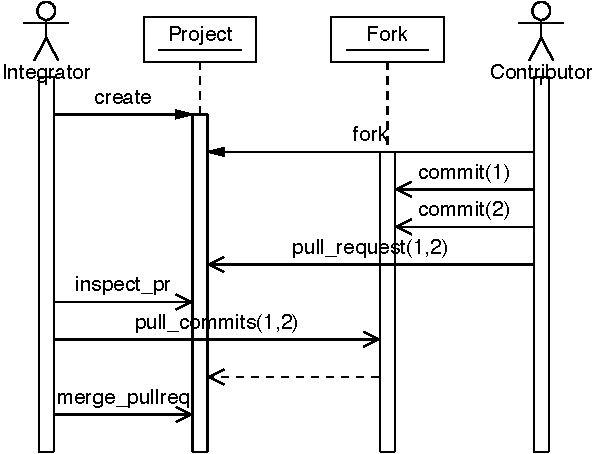
\includegraphics[scale=0.5]{pullreq}
      \end{center}
      \caption{The pull request process.}
      \label{fig:pullreq-process}
    \end{figure}

\subsection{Pull requests on Github}

Github supports all types of distributed development outlined above; however,
pull requests receive special treatment. The site is tuned to allow easy forking
of projects by contributors, while automating the generation of pull requests
through automatic comparison of project branches.
Github's pull request model follows the generic pattern presented above; in
addition it provides tools for contextual discussions and in-line code reviews.
An example pull request on Github can be seen in Figure~\ref{fig:pullreq-scr}.

\begin{figure}[t]
  \centering
   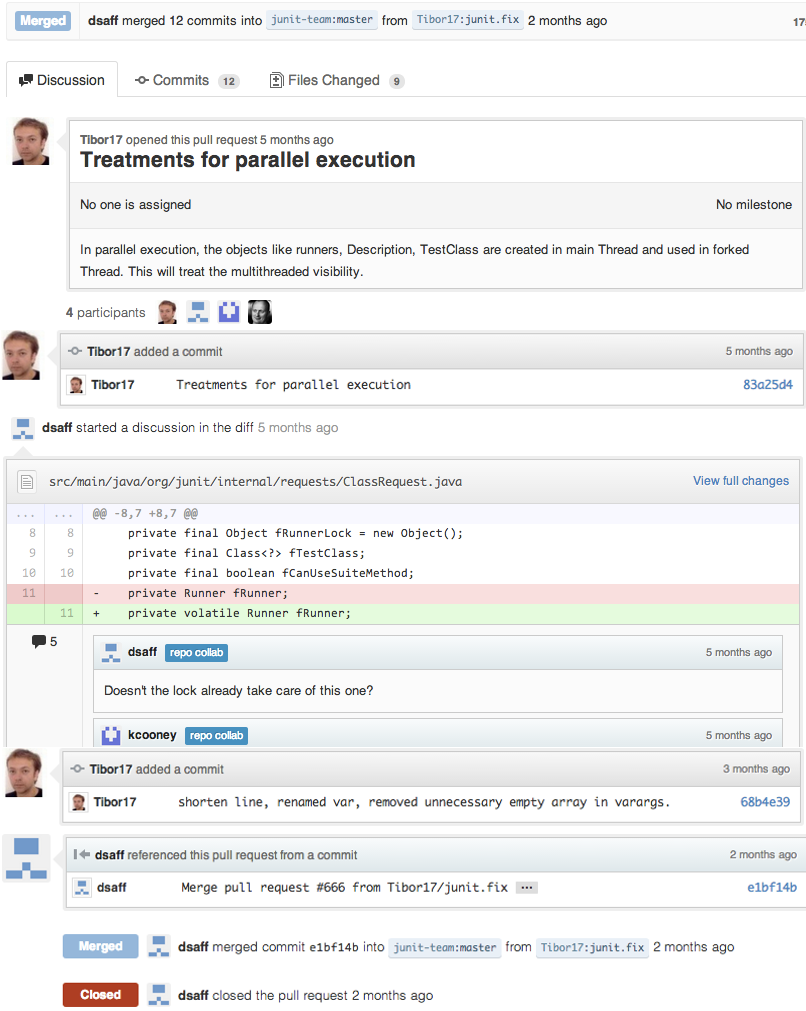
\includegraphics[scale=0.23]{pullreq-scr.png}
   \label{fig:pullreq-scr}

   \caption{An example Github cross-branch pull request (edited for space). The
   participants first interact in several code reviews, the result of which is
   the update of the pull request. The second reviewer then approves the pull
   request, which is merged by the author.}

\end{figure}

A Github pull request contains a branch (local or in another repository) from
which a core team member should pull commits from. Github automatically
discovers the commits to be merged and presents them in the pull request. By
default, pull requests are submitted to the base repository for inspection. The
inspection is either a code review of the commits submitted with the pull
request or a discussion about the features introduced by the pull request. Any
Github user can participate to both types of inspection. As a result of the
inspection, pull requests can be updated with new commits or be closed as
redundant, uninteresting or duplicate. In case of an update, the pull request
creator creates new commits in the forked repository, while Github automatically
updates the displayed commits. The code inspection can then be repeated on the
refreshed commits.

When the inspection process finishes and the pull requests are deemed
satisfactory, the pull request can be merged. A pull request can only be merged
by core team members. The versatility of Git enables pull requests to be
merged in various ways, presented below sorted by the amount of preservation of
the original source code properties:

\textbf{Through Github facilities.}
    Github can automatically verify whether a
    pull request can be merged without conflicts to the base repository. When a
    merge is requested, Github will automatically apply the commits in the pull
    request and record the merge event. All authorship and history information
    is maintained in the merged commits.

\textbf{Using Git merge.} When a pull request cannot be applied cleanly or
    when project-related policies do not permit automatic merging, a pull
    request can be merged using plain Git utilities, using the following
    techniques: 

    \begin{itemize}

      \item \emph{Branch merging:} The remote branch containing the pull
        request commits is added as a source to a local repository. The remote 
        branch is merged to a local upstream branch, which is then pushed to
        the central repository or published for further pulling by other
        developers. Both history and authorship information are maintained,
        but Github cannot detect the merge in order to record a merge
        event~\cite[Chapter 3.2]{Chaco09}. 

      \item \emph{Cherry-picking:} Instead of merging all commits, the merger
        picks specific commits from the remote branch, which then applies to the
        upstream branch. The commit unique identifier changes, so exact history
        cannot be maintained, but authorship is 
        preserved~\cite[Chapter 5.3]{Chaco09}.
    
    \end{itemize}

    A technique that complements both of the above is \emph{commit
    squashing}: when the full history is not of interest to the project,
    several consecutive commits are merged into a single one on the pull request
    branch, which can then be merged or cherry-picked to the upstream branch. In
    this case, the author of the commit can be different from the person that
    applied the commit~\cite[Chapter 6.4]{Chaco09}.

\textbf{Committing the patch.} 
  The merger creates a textual difference between the upstream and the pull
  request branch, which she then applies to the upstream branch. Both history and
  authorship information are lost.

As the project branches are updated in a distributed manner, the changes in a
pull request may interfere with new changes in the project's main branch. Merging
such a pull request will result to \emph{conflicts}. Github automatically
detects conflicting pull requests and marks them as such. Conflicts can be
resolved by either the contributor or a core team member; however, pull request
etiquette dictates resolving the conflicts at the contributor's site. The
conflict resolution process involves pulling new commits from the project's main
repository, resolve the conflicts and upgrading the pull request with the a new
merge commit.

Issues and pull requests are dual on Github; for each pull request, an issue is
opened automatically. Commits can also be attached to issues to convert them to
pull requests (albeit with external tools). This duality enables project administrators to treat pull requests as work items, which can be managed using the same facilities used for issues. Moreover, issue discussions can include
links to pull requests and vice versa, while specific message formats can be used
in commit comments to automatically close issues or pull requests when commits
are merged to the project's main branch.

The open nature of Github's pull requests lends itself to a variety of usage
patterns. Except from basic patch submission, pull requests can be used as a
requirements and design discussion tool\footnote{Github uses this internally:
\url{https://github.com/blog/1124-how-we-use-pull-requests-to-build-github}} or
as a progress tracking tool towards the fulfilment of a project
release.\footnote{\url{https://github.com/blog/831-issues-2-0-the-next-generation}} In
the first case, a pull request serves as a discussion board for soliciting the
opinions of other developers while a new feature is being implemented. In the
second case, pull requests are associated with milestones in Github's issue
tracker.

\section{Research Design}

The main focus of this study is to understand and explain how pull requests are
used by projects to enable collaboration. To answer our research questions, we
use a sequential mixed-methods approach. Mixed methods is a procedure for
collecting, analyzing, and integrating both quantitative and qualitative data at
some stage of the research process within a single study for the purpose of
gaining a better understanding of the problem~\cite{Ivank06}. For specific 
research questions, we first explore the domain quantitatively,
and then highlight specific interesting cases by exploring cases qualitatively.

We present here how we analyzed each 

{\bfseries RQ1} To assess the popularity of the pull-based development model, we
provide and analyze descriptive statistics on the use of pull request in Github.
In particular, we investigate such questions as how many projects actually make
use of pull requests, how many of the projects are original repositories
(versus, e.g., clones), and what the relation is to Github's issue tracking
facilities is. The outcomes are in Section~\ref{sec:ghtorrent}.

{\bfseries RQ2 and RQ3} Answering {\sc rq2} and {\sc rq3} first of all requires
a dedicated dataset of projects that have a sufficiently long history of using
pull requests. This dataset is described in Section~\ref{sec:expdata}.

Given this dataset, we answer {\sc rq2} and {\sc rq3} by determining a set of
suitable candidate features by consulting related work in the fields of patch
submission and bug triaging. Then, we clean it up through cross-correlation
analysis to obtain a set of features with maximum predictive power
(Section~\ref{sec:featureselection}). Using the extracted data for the extracted
features, we perform a detailed statistical analysis of pull request
characteristics to answer {\sc rq2}  (Section~\ref{sec:pullreqchar}).

Using the identified features, we use machine learning to retrieve
the dominant ones. Prior to running the classification algorithms, we labeled
each pull request with an outcome factor; in the case of the \textsf{merge
decision} classification task, the factor signifies whether the pull request
has been merged. For the \textsf{merge time} task, we first filter out pull
requests that have not been merged and then split the remaining data points in
three bins (one hour, one day and remaining) according to the time 
required to merge the pull request. The bins were chosen to reflect the
results of {\sc rq2}, and split the available data points in roughly
equally sized bins.

At a high level, the process to retrieve the dominant features for both
problems consists of two steps: i) we run each dataset through 3 well known
classification algorithms, namely Random Forests (\texttt{randomforest}),
variants of Logistic Regression (\texttt{logregr}) (binary for the \textsf{merge decision} task, multinomial for the \textsf{merge time} task) and Na\"ive Bayes (\texttt{naivebayes}), and ii) we select
the best classifier and apply a classifier-specific process to extract the
feature importance. 

To evaluate the classification performance, we used the Accuracy ({\sc acc}) and
Area Under the receiver operating characteristic Curve ({\sc auc}) metrics. To
select the appropriate classification algorithm, we run a 10-fold random
selection cross-validation and aggregate the mean values for each classification
metric. At each iteration, the algorithm randomly samples 10,000 data points
from the whole dataset, train a classifier with 90\% percent of the input and
use it to predict the remaining 10\%. The 10-fold run results also allowed us to
evaluate the metric stability across runs. We did not perform any additional
tuning to the classification algorithms (Section~\ref{sec:accrej}).

{\bfseries RQ4} Applying machine learning to answer {\sc rq4} would pose a
significant challenge, as the lack of a standardized way of processing pull
requests across projects hinders our ability to extract reliable relevant
features. We therefore opted to do in-depth qualitative analysis of a limited
number of random chosen pull requests. We used grounded coding to come up with
an inclusive set of tags of why pull requests are not merged as follows: The
first author read the pull request discussion on Github and summarized it into
one sentence per sample; during the second pass, the descriptions were
aggregated and codes were extracted. To validate the identified codes, all three
authors applied them on a different set of pull requests, compared results and
identified inconsistencies. The final set of codes was applied on a third sample
and we used that sample to draw results from. The sampling process is described
in Section~\ref{sec:qualitative}.

{\bfseries Replication}This study has been conducted using the {\sc ght}orrent
dataset and custom-built Ruby and R tools. We share the tools, original data
sources and extracted data files on the Github repository
\texttt{gousiosg\-/\-pullreqs}. The execution of all tools is scripted and it is
possible to run it in sequence automatically.

\section{Data}

\subsection{Github Data}
\label{sec:ghtorrent}
For both phases, we use data obtained through the Github \api.
In particular, we do this by means of the \ghtorrent
dataset~\cite{GS12}.
%
\ghtorrent is  an off-line mirror of the data
offered through the Github {\sc api}. The Github {\sc api} 
data come in two forms; a streaming
data flow lists events, such as forking or creating pull requests, happening on
repositories in real time, while a static view contains the current state of
entities. To obtain references to the roots of the static view entities, the
{\sc ght}orrent project follows the event stream. From there, it applies a
recursive dependency-based parsing approach to yield all data offered through
the {\sc api}. The data is stored in unprocessed format, in a Mongo{\sc db}
database, while metadata is extracted and stored in a My{\sc sql} relational
database. The {\sc ght}orrent dataset covers a broad range of development
activities on Github, including pull requests and issues. Up to August 2013,
1.8 million pull requests from more that two hundred thousand projects
have been collected.

\subsection{Pull request project sample}
\label{sec:expdata} 

While an overview of pull request activity can be safely extracted from the \ghtorrent dataset, several limitations do not allow us to apply our detailed
analysis across all projects. Specifically, projects worth analyzing have a
history longer than 1$\sfrac{1}{2}$ years, the data collection period of \ghtorrent, and it is important to retrieve all information
available during the project's life. To make the data collection and subsequent
analysis practical we use a dataset consisting of all projects for which
GHTorrent recorded more than 200 pull requests since January 2012. The
following inclusion criteria were then specified:

\begin{itemize}

  \item Projects should include tests. To measure the effect of testing on pull
    request acceptance, we could only use projects that include tests which we
    could measure reliably. For that, we exploited the convention-based project
    layout in the Ruby (Gem), Python, Java and Scala (both Maven) language
    ecosystems, so our project selection was limited to those languages. 

  \item Projects should have a committer count larger than the main team member
    count, to ensure that the project is open to external contributions and that
    pull requests are indeed used by developers outside the project.

  \item Projects should be developing software frameworks or applications,
    rather than documentation or programming languages. We excluded
    documentation projects, because we are interested in distributed software
    development. We excluded programming language implementation projects
    because we wanted to avoid cases where the developed programming language's
    core library was overshadowing the metrics of the actual implementation.
    This is especially true for the 5 Ruby implementations hosted on Github.

\end{itemize}

After selection, the full history (including pull requests, issues and commits)
of the included projects was downloaded and features were extracted by querying
the {\sc ght}orrent databases and analysing each project's Git repository. To
compensate for pull requests that are merged outside Github, which Github
reports as unmerged, we resorted to the following heuristics, listed here in
order of application:

\begin{itemize}

  \item At least one of the commits associated with the pull request appears in
    the target project's master branch. 

  \item A commit closes the pull request (using the \texttt{fixes: } convention
    advocated by Github) and that commit appears in the project's master branch.
    This means that the pull request commits where squashed into one commit and
    this commit was merged.

  \item The last 3 (in order of appearance) discussion comments contain
    a commit unique identifier, this commit appears in the
    project's master branch and the comment can be matched by the following 
    regular expression:

    \texttt{merg(?:ing|ed)|appl(?:ying|ied)|\-
            pull[?:ing|ed]|push[?:ing|ed]|\-
            integrat[?:ing|ed]}

  \item The latest comment prior to closing the pull request matches the 
    regular expression above.

\end{itemize}

If none of the above heuristics identifies a merge, we mark the pull request
as unmerged. 

After creating the data files, we investigated cases where the pull request
merge ratio was significantly less than the one we calculated across Github
(73\%), and in any case less than 40\%, as this means that our heuristics are not
inclusive enough. This way, we filtered out 2 projects, which we did not
replace.

The final dataset consisted of 291 projects (99 Python, 91 Java, 87 Ruby, 14
Scala) and 166,737 data points (59,970, 55,320, 43,871 and 7,576 for Python,
Ruby, Java and Scala projects respectively). Both distributions are
representative of the contemporary popularity of each respective programming
language on both Github and other sites.

%Figure~\ref{fig:wordcloud} presents the project names in relative size to the
%pull requests included per project in the dataset. 
%
%\begin{figure}
%  \begin{center}
%    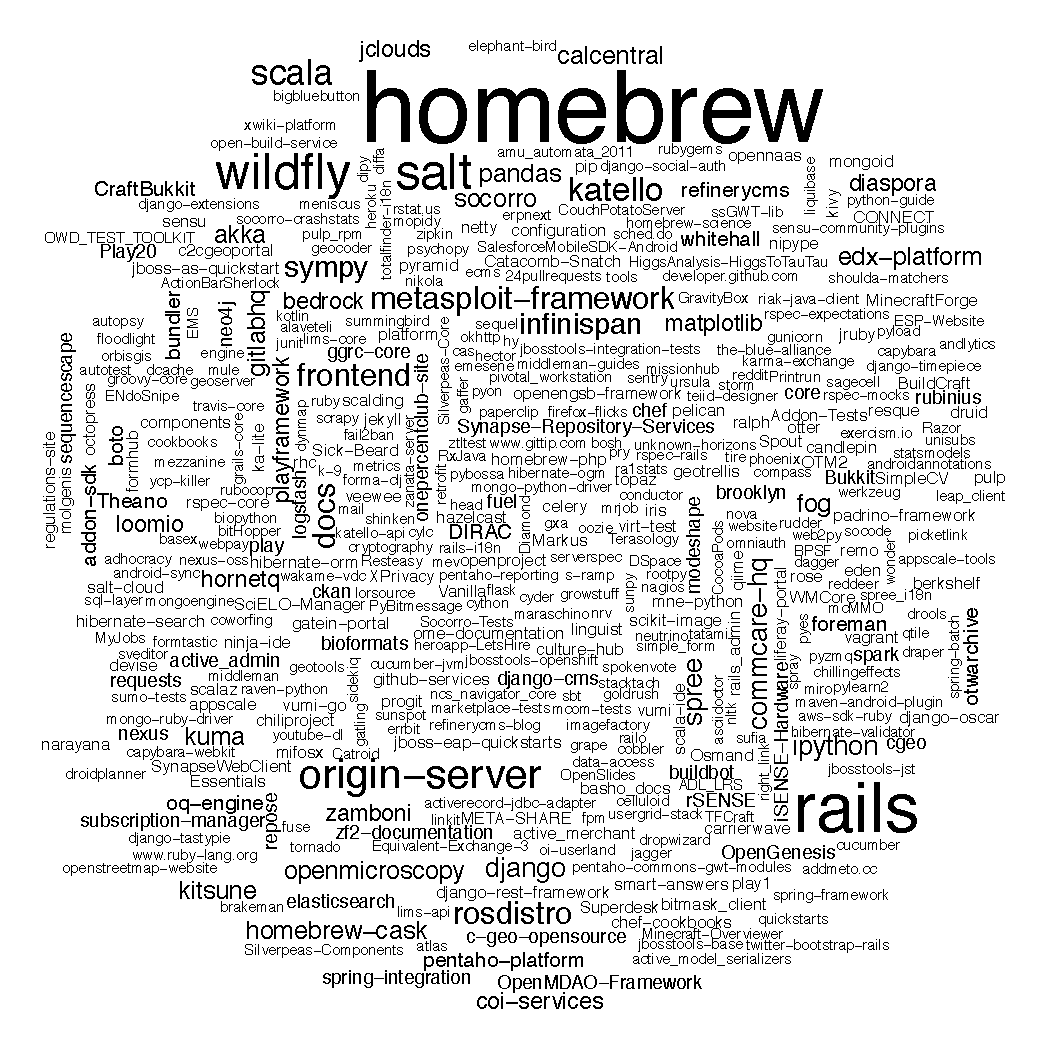
\includegraphics[scale=0.7]{wordcloud.pdf}
%  \end{center}
%  \caption{Projects in our dataset. Text size is relative to the number of
%  included pull requests.}
%  \label{fig:wordcloud}
%\end{figure}

\textbf{Feature Extraction} The feature selection was based on prior work in the areas of patch submission
and acceptance~\cite{Nagap05,Bird07a,Weiss08,Baysa12}, bug
triaging~\cite{Anvik06, Giger10} and also on the semi-structured interviews of
Github developers in Pham et al.~\cite{Pham13}. The selected features are split
in three categories:

  \emph{Pull request impact.} These
    features attempt to quantify the impact of the
    pull request on the affected code base. When examining external code
    contributions, the size of the patch is affecting both acceptance and
    acceptance time~\cite{Weiss08}. There are various metrics to determine the
    size of a patch that have been used by researchers: code
    churn~\cite{Nagap05, Ratzi07}, changed files~\cite{Nagap05} and number of
    commits~\cite{Fluri07}. In the particular case of pull requests, developers
    reported that tests in a pull request increases their confidence to merge
    it~\cite{Pham13}. To investigate this, we split the churn feature to two
    features, namely \texttt{src\_churn} and \texttt{test\_churn}.

  \emph{Project characteristics.} These features quantify how receptive to pull
  requests the project is. If the project's process is open to external
  contributions, then we expect to see an increased ratio of external
  contributors over team members. The project's size may be a detrimental factor
  to the speed of processing a pull request, as its impact may be more difficult
  to assess. Also, incoming changes tend to cluster over time (the
  ``yesterday's weather'' change pattern~\cite{Girba04}), so it is natural to
  assume that pull requests affecting a part of the system that is under active
  development will be more likely to merge. Testing plays a role in speed of
  processing; according to~\cite{Pham13}, projects struggling with constant flux
  of contributors use testing, manual or preferably automated, a safety net to
  handle contributions from unknown developers.

  \emph{Developer.}  
    Developer-based features quantify the influence that the person that
    created the pull request has on the decision to merge it and
    the time to process it. In particular, the developer that created the patch
    has been shown to influence the patch acceptance decision~\cite{Jeong09}. To
    abstract the results across projects with different developers, we
    include features that quantify the developer's track record, namely the
    number of previous pull requests and their acceptance rate; the former has
    been indicated as a strong indicator of pull request quality~\cite{Pham13}.
    Bird et al.~\cite{Bird07}, presented evidence that social
    reputation has an impact on whether a patch will be merged; in our dataset,
    the number of followers on Github is an interesting proxy for
    reputation.

All features are calculated at the time a pull request has been closed or
merged, to evaluate the effect of intermediate updates to the pull request as a
result of the ensuing discussion. Features that contain a temporal dimension in
their calculation (e.g., \texttt{team\_size} or
\texttt{commits\_on\_files\_touched}) are calculated in a time window of $t - 3$
months, where $t$ is the time the pull request has been closed. 

The initial selection contained 23 features. To check whe\-ther the selected
features are independent enough, and therefore have strong explanatory power, we
conducted a pair-wise correlation analysis using the Spearman rank correlation
($\rho$) metric across all features. We set a threshold of $\rho = 0.7$, above
which we eliminated features that are strongly correlated. Using this cutoff, we
removed 2 features, \texttt{asserts\_per\_kloc} and
\texttt{test\_cases\_per\_kloc} as they where very strongly correlated ($\rho >
0.92$) with the included \texttt{test\_lines\_per\_kloc} feature. We also
removed features that could not be calculated reliably at the time a pull
request was done (\texttt{followers} and \texttt{stars}).\footnote{The Github
{\sc api} does not report a timestamp on when a user followed another user, or
when a user stared a project, so it is impossible to know how many followers a
user had or stars a project had at a specific time instance.} Finally, we
merged similar features (i.e. \texttt{doc\_files} and \texttt{src\_files} were merged to \texttt{files\_changed}). 

The post processing phase left us with 13 features, which can be seen in
Table~\ref{tab:features}. The cross-correlation analysis result for the
selected features can be seen in Figure~\ref{fig:crosscor}. In general, very few
features are correlated at a value $\rho > 0.2$, while only two,
\texttt{src\_churn} and \texttt{files\_changed}, are strongly correlated at
$\rho = 0.63$. While the correlation is strong, it is below our threshold and it
is not definite; therefore we do not remove either feature from the dataset. All
results are statistically significant ($n = 166,737, p < 0.001$).

%\begin{table*}
%  \begin{small}
%  \centering
%  \begin{tabular}{rp{40em}}
%    \hline
%    \bf{Feature} & \bf{Description and Justification}\\
%    \hline
%    \multicolumn{2}{l}{\bf{Pull Request Impact}}\\
%    
%    \texttt{num\_commits} & Number of commits in the pull request. A bigger
%    pull request should be slower to examine and therefore to merge.\\
%    
%    \texttt{src\_churn} & Number of lines changed (added + deleted) by the pull
%    request. The more lines changed, the longer a pull request should take to be
%    reviewed.\\
%
%    \texttt{test\_churn} & Number of test lines changed in the pull request. Pull requests
%    that include tests should be faster to merge, as testing would increase
%    confidence for the merger.\\
%    
%    \texttt{files\_changed} & Number of files touched by the pull request. An
%    indication of the impact of the pull request.\\
%    
%    \texttt{num\_comments} & The total number of comments (discussion and code
%    review). More pull code review comments may indicate a rigorous process,
%    therefore slowing down acceptance.\\
%
%    \texttt{conflict} & The word conflict appears in the pull request comments.
%    Pull request that conflict with other branches should be slower to merge.\\
%
%    \texttt{forward\_link} & The pull request comments include links to other
%    pull requests. Pull requests with forward links should be overridden by
%    other pull requests and therefore not merged.\\
%
%    \multicolumn{2}{l}{\bf{Project Characteristics}}\\
%    
%    \texttt{sloc} & Executable lines of code at pull request merge time. The
%    bigger the project, the more difficult would be to assess the impact of
%    a pull request. \\
%
%    \texttt{team\_size} & Number of active core team members during the last 3
%    months prior the pull request creation. A big team will be faster to process
%    a pull request as each team member will have less work load to handle and
%    will be more specialized.\\
%
%    \texttt{perc\_external\_contribs} & The ratio of commits from external
%    members over core team members in the last 3 months prior to pull request
%    creation. A higher ratio indicates a more open
%    process, which may lead to more accepted pull requests.\\
%
%    \texttt{commits\_on\_files\_touched} & Number of total commits on files
%    touched by the pull request 3 months before the pull request creation time.
%    If the pull request touches files in a hotspot, it will be merged faster.\\
% 
%    \texttt{test\_lines\_per\_1000\_lines} & A proxy for the project's test
%    coverage. The more well tested a project is, the faster a pull request
%    could be merged, as applying it and testing its impact would be faster. \\
%
%    \multicolumn{2}{l}{\bf{Developer}}\\
%    
%    \texttt{prev\_pullreqs} & Number of pull requests submitted by a specific
%    developer, prior to the examined pull request. The more pull requests, the
%    better the developer is known to the project.\\
%
%    \texttt{requester\_succ\_rate} & The percentage of the developer's pull requests that have been merged up to the creation of the examined pull
%    request. A high success rate indicates a developer trusted by the project.\\
%
%    \texttt{main\_team\_member} & Whether the developer belongs to the
%    main repository team. Pull requests from main team members should be
%    faster to accept and merge due to increased confidence.\\
%    \hline
%  \end{tabular}
%  \caption{Selected features and intuition driving the selection.}
%  \label{tab:features}
%  \end{small}
%\end{table*}
%

% latex table generated in R 2.15.3 by xtable 1.7-1 package
% Sat Jan 11 16:56:59 2014
\begin{table*}
\centering
\begin{tabular}{rp{20em}rrrrc}
  \hline
  \bfseries{Feature} & \bfseries{Description} & \bfseries{5\%} & \bfseries{mean} & \bfseries{median} & \bfseries{95\%} & \bfseries{histogram} \\ 
  \hline
   \multicolumn{2}{l}{\bf{Pull Request Characteristics}}\\
lifetime\_minutes & Minutes between opening and closing & 0.00 & 15,418 & 581.00 & 72,508 & 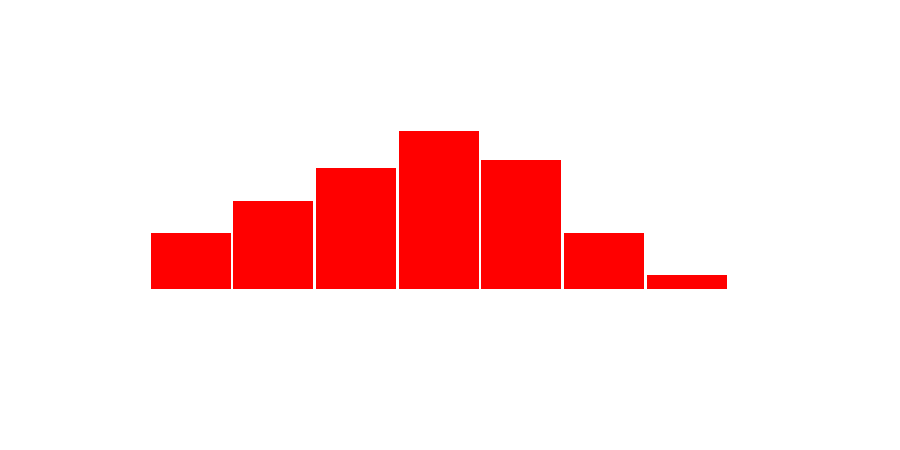
\includegraphics[scale = 0.1, clip = true, trim= 50px 60px 50px 60px]{hist-29b6fa715eecc1dad108c8148465533b.pdf} \\ 
  mergetime\_minutes & Minutes between opening and merging (only for merged pull
    requests) & 0.00 & 10,506 & 418.00 & 44,234 & 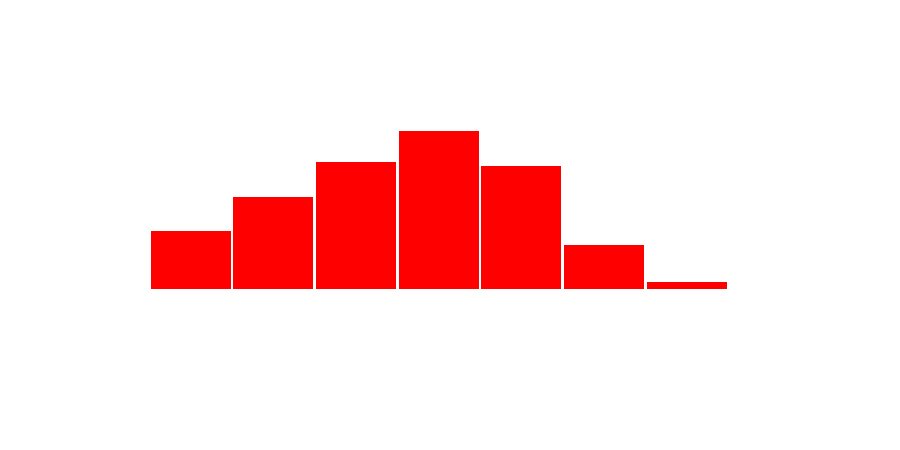
\includegraphics[scale = 0.1, clip = true, trim= 50px 60px 50px 60px]{hist-e2ded77f4080f561e112a1f363b125ce.pdf} \\ 
  num\_commits & Number of commits & 1.00 & 4.42 & 1.00 & 12.00 & 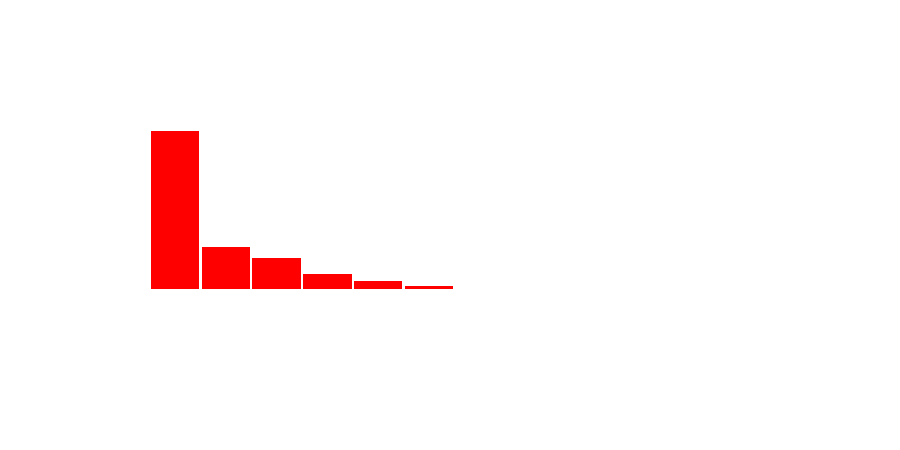
\includegraphics[scale = 0.1, clip = true, trim= 50px 60px 50px 60px]{hist-f128f3cb38588fe5202716588c047381.pdf} \\ 
  src\_churn & Number of lines changed (added + deleted) & 0.00 & 282.95 & 10.00 & 846.00 & 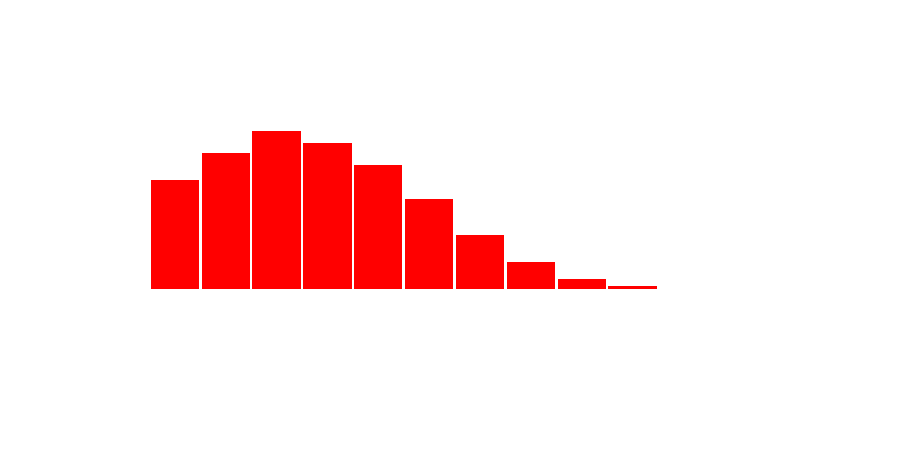
\includegraphics[scale = 0.1, clip = true, trim= 50px 60px 50px 60px]{hist-1f006c80a0da61518435a0c55f538326.pdf} \\ 
  test\_churn & Number of test lines changed & 0.00 & 79.74 & 0.00 & 248.00 & 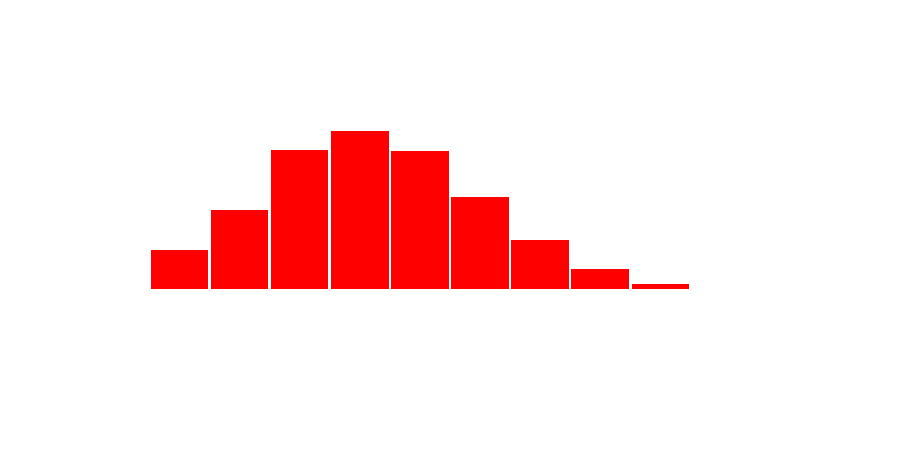
\includegraphics[scale = 0.1, clip = true, trim= 50px 60px 50px 60px]{hist-dd78ccaeedd7fc79735a66eb7f9e506b.pdf} \\ 
  files\_added & Number of files added  & 0.00 & 4.01 & 0.00 & 7.00 & 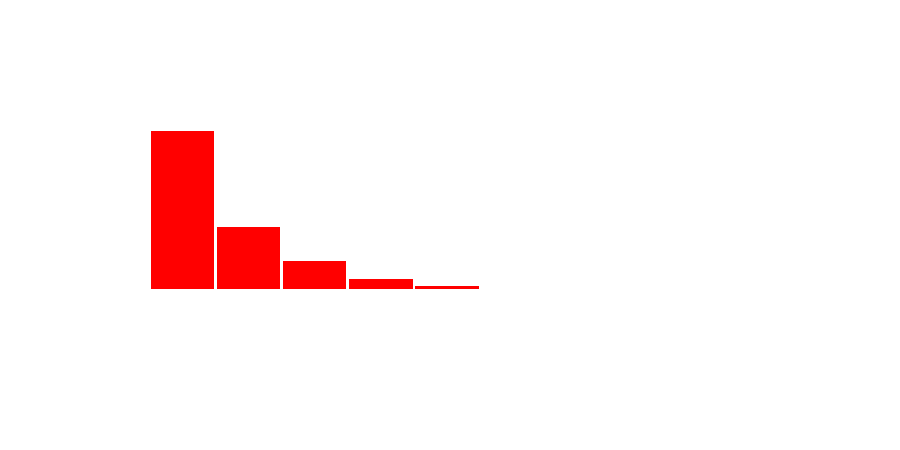
\includegraphics[scale = 0.1, clip = true, trim= 50px 60px 50px 60px]{hist-340be33adc9a51666460c68028842c1d.pdf} \\ 
  files\_deleted & Number of files deleted  & 0.00 & 2.05 & 0.00 & 1.00 & \includegraphics[scale = 0.1, clip = true, trim= 50px 60px 50px 60px]{hist-bd564691a0c6275ea5f30bcc0b81b3f5.pdf} \\ 
  files\_modified & Number of files modified  & 1.00 & 7.56 & 2.00 & 21.00 & 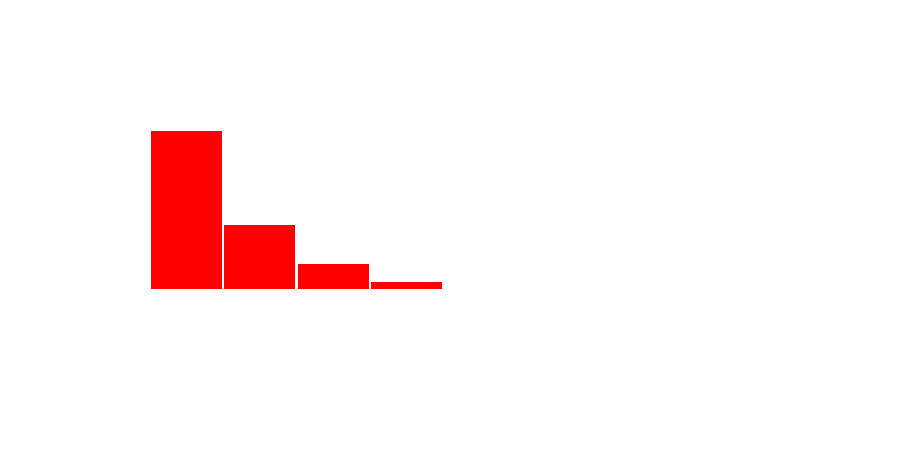
\includegraphics[scale = 0.1, clip = true, trim= 50px 60px 50px 60px]{hist-52a19dc5ca5e4f8c5325bca43137a6c1.pdf} \\ 
  files\_changed & Number of files touched (sum of the above) & 1.00 & 13.62 & 2.00 & 32.00 & 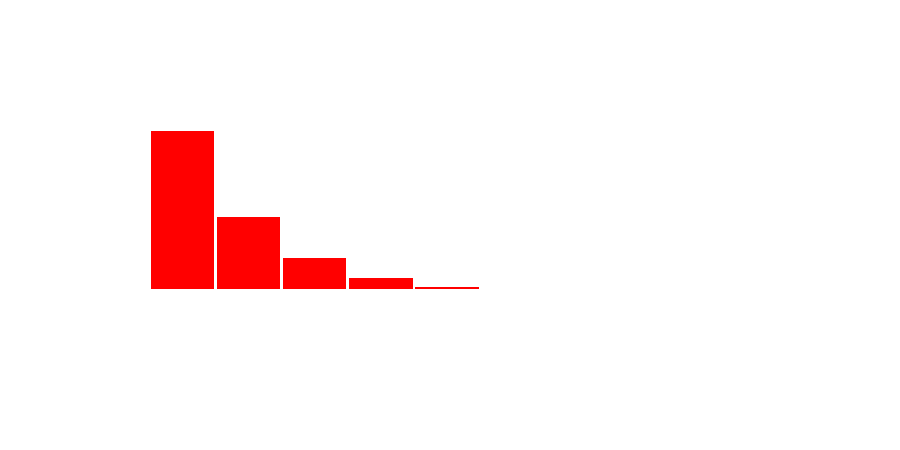
\includegraphics[scale = 0.1, clip = true, trim= 50px 60px 50px 60px]{hist-9b07b060359435635ff2bf4cd34f834a.pdf} \\ 
  src\_files & Number of source code files touched by the pull request & 0.00 & 7.64 & 1.00 & 20.00 & 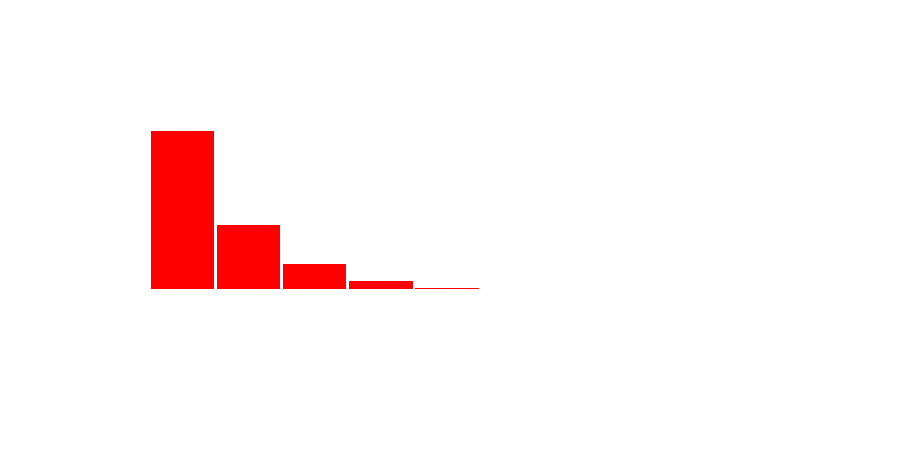
\includegraphics[scale = 0.1, clip = true, trim= 50px 60px 50px 60px]{hist-2d4e53ba8eec29c0c79c1e834756c654.pdf} \\ 
  doc\_files & Number of documentation (markup) files touched & 0.00 & 2.36 & 0.00 & 6.00 & 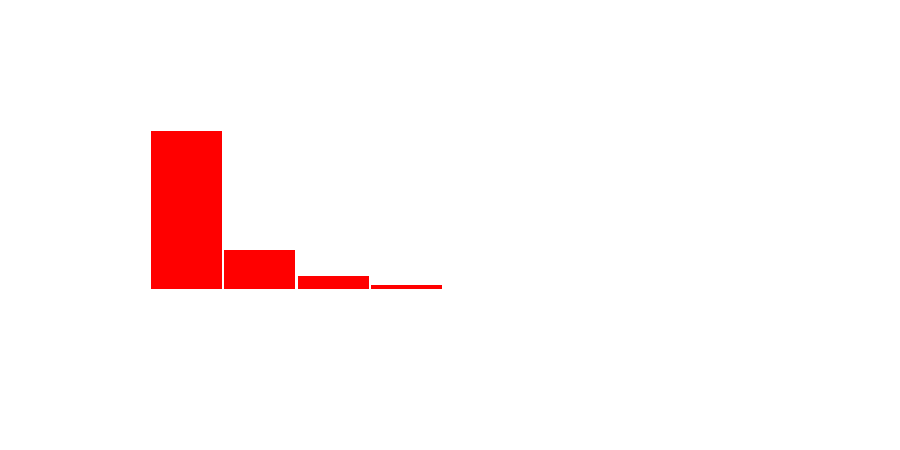
\includegraphics[scale = 0.1, clip = true, trim= 50px 60px 50px 60px]{hist-d4fb585969e7acb86dd568d80e7f1500.pdf} \\ 
  other\_files & Number of non-source, non-documentation files touched & 0.00 & 2.74 & 0.00 & 4.00 & 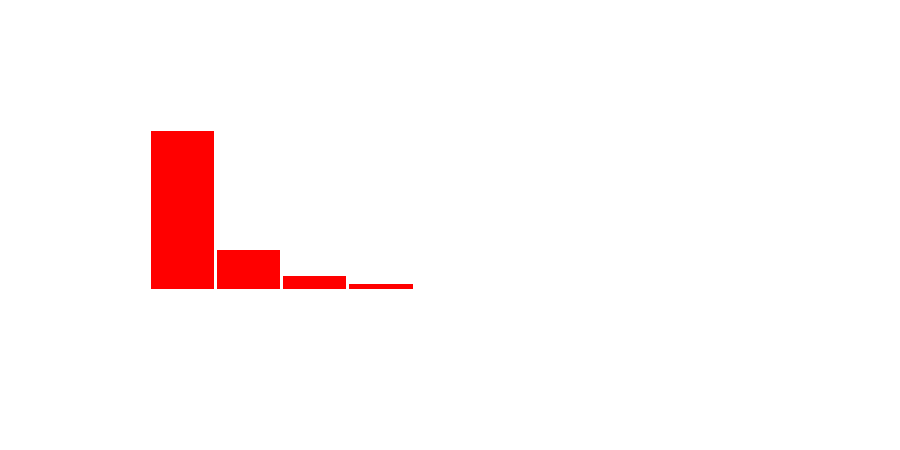
\includegraphics[scale = 0.1, clip = true, trim= 50px 60px 50px 60px]{hist-df965fcd0b03a96f1b31b2eda13d2b98.pdf} \\ 
  num\_commit\_comments & The total number of code review comments & 0.00 & 0.73 & 0.00 & 4.00 & 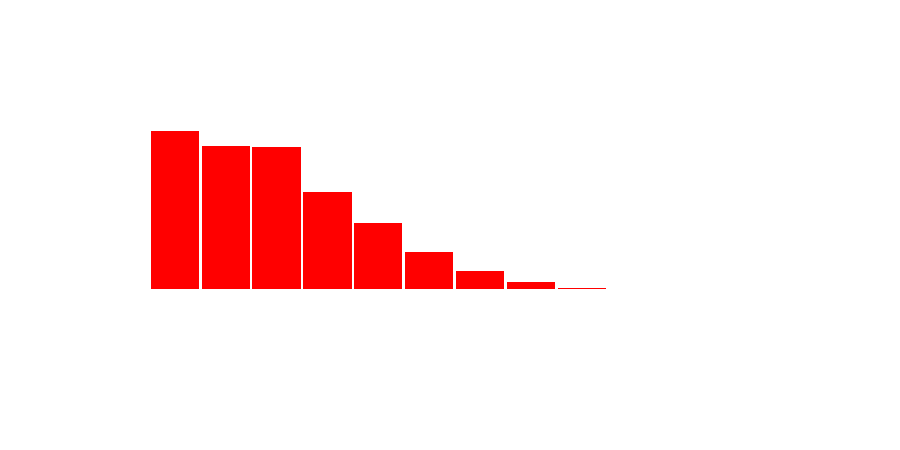
\includegraphics[scale = 0.1, clip = true, trim= 50px 60px 50px 60px]{hist-f0fac61db5a83629be8f04cc84e8b907.pdf} \\ 
  num\_issue\_comments & The total number of discussion comments & 0.00 & 1.84 & 0.00 & 8.00 & 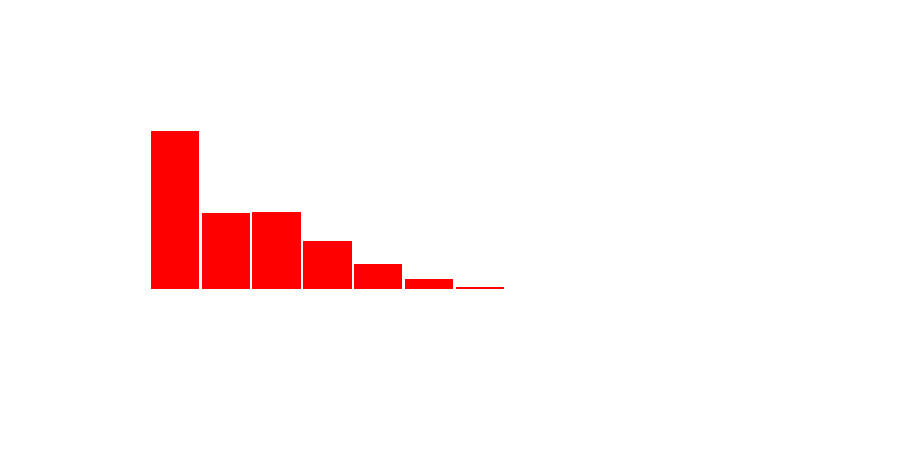
\includegraphics[scale = 0.1, clip = true, trim= 50px 60px 50px 60px]{hist-fee6653ed7b2359f7e7374841378492b.pdf} \\ 
  num\_comments & The total number of comments (discussion and code review). & 0.00 & 2.57 & 1.00 & 11.00 & 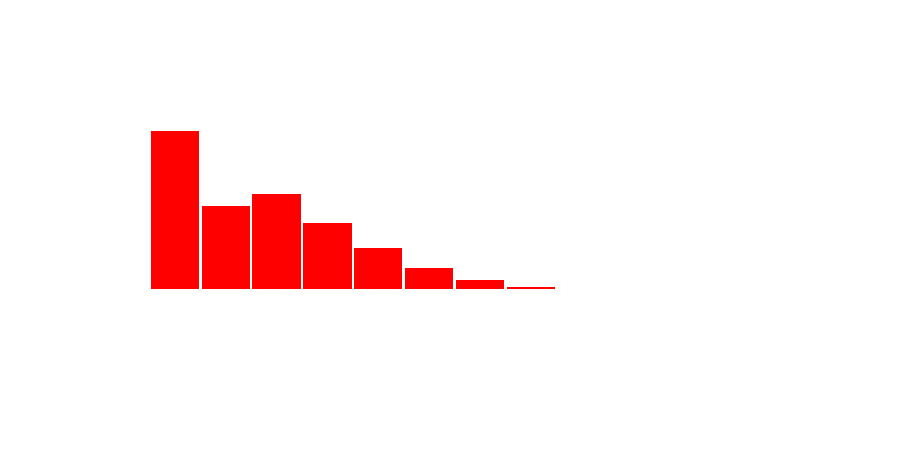
\includegraphics[scale = 0.1, clip = true, trim= 50px 60px 50px 60px]{hist-9db5e2b390de0d64d26c14798cb579ef.pdf} \\ 
  num\_participants & Number of participants in the discussion & 0.00 & 1.27 & 1.00 & 4.00 & 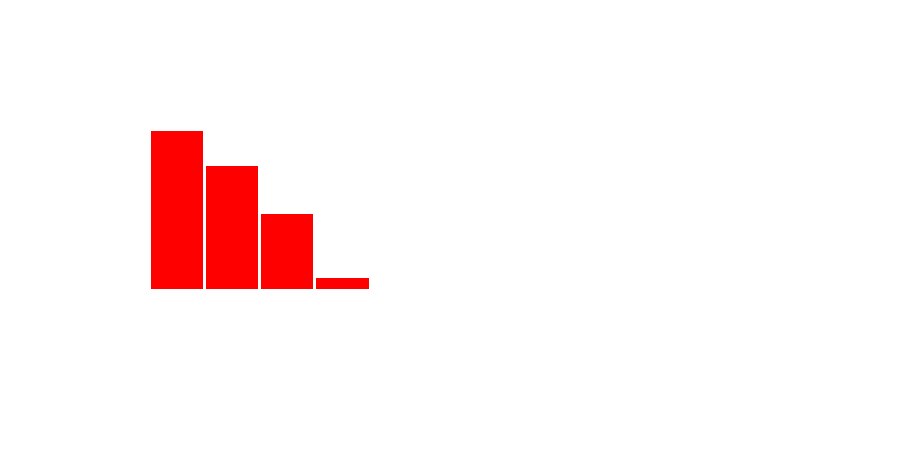
\includegraphics[scale = 0.1, clip = true, trim= 50px 60px 50px 60px]{hist-7d419bb69f175ea7015a9bdc71172f38.pdf} \\ 
  \multicolumn{2}{l}{\bf{Project Characteristics}}\\
  
  sloc & Executable lines of code at creation time. & 458.00 & 53,801 & 18,019 & 275,058 & 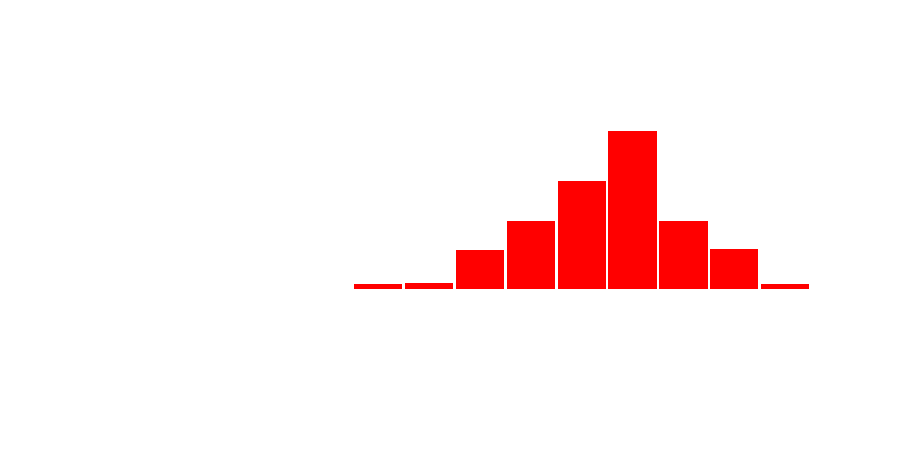
\includegraphics[scale = 0.1, clip = true, trim= 50px 60px 50px 60px]{hist-6b5159d3060b4fdf8493d4c818f79949.pdf} \\ 
  team\_size & Number of active core team members during the last 3 months prior to creation. & 1.00 & 20.64 & 7.00 & 93.00 & 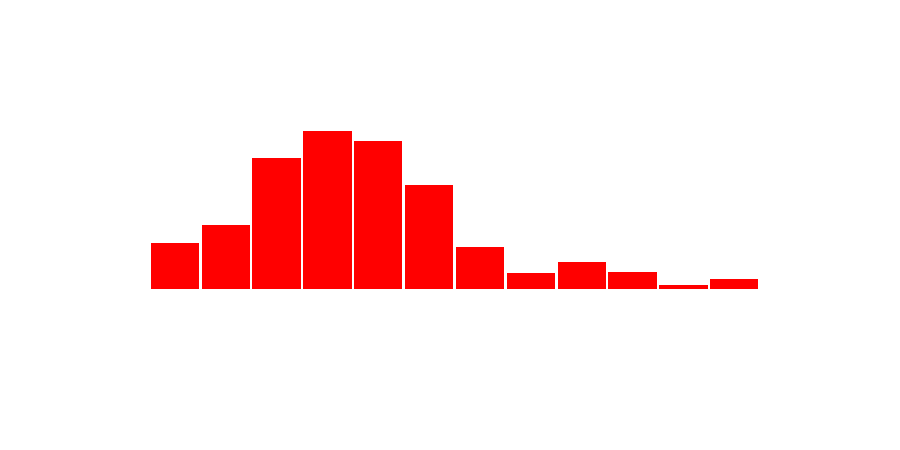
\includegraphics[scale = 0.1, clip = true, trim= 50px 60px 50px 60px]{hist-231fb4fabf4a3f0c551f2a97ae080508.pdf} \\ 
  perc\_external\_contribs & The ratio of commits from external members over core team members in the last 3 months prior to creation. & 8.00 & 54.01 & 56.00 & 95.00 & 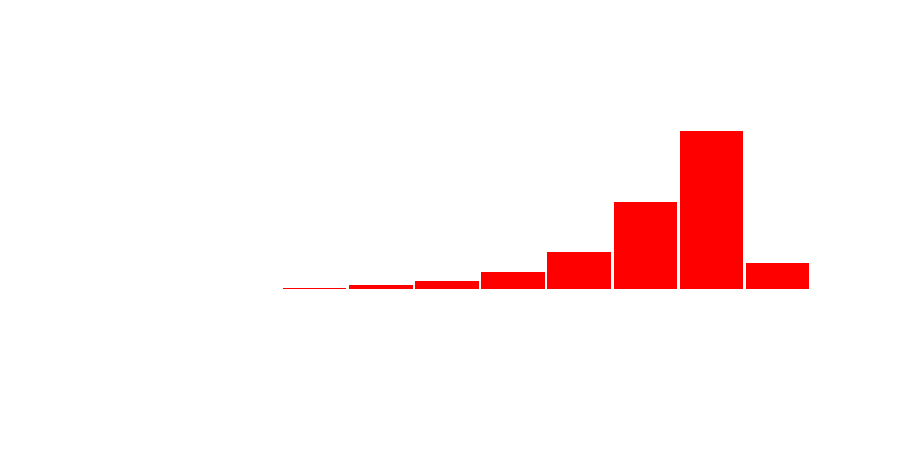
\includegraphics[scale = 0.1, clip = true, trim= 50px 60px 50px 60px]{hist-a222f0a5c377ba129dd6c8f257062591.pdf} \\ 
  commits\_on\_files\_touched & Number of total commits on files touched by the pull request 3 months before the creation time. & 0.00 & 51.65 & 4.00 & 209.00 & 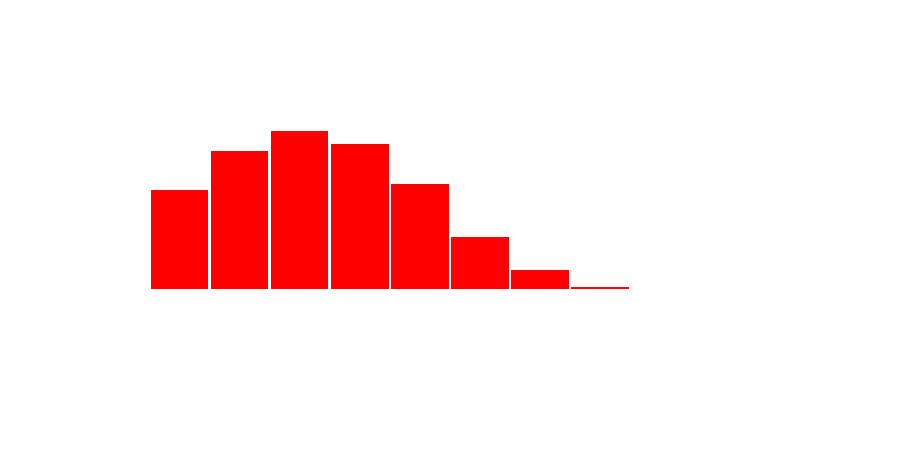
\includegraphics[scale = 0.1, clip = true, trim= 50px 60px 50px 60px]{hist-b735900ffcc37e7eda16dcd0c3497e6e.pdf} \\ 
  test\_lines\_per\_kloc & Executable lines of test code per 1,000 lines of source code & 0.00 & 1,297 & 355.21 & 2,097 & 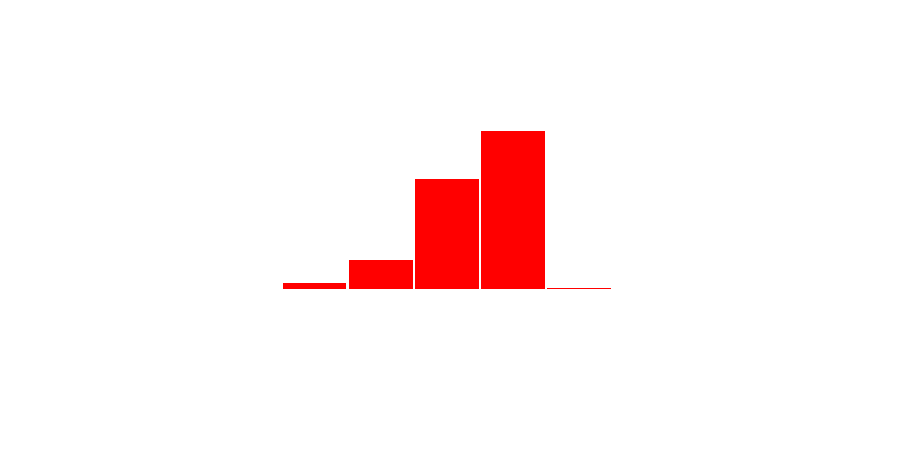
\includegraphics[scale = 0.1, clip = true, trim= 50px 60px 50px 60px]{hist-67ff3047089ba9ce0528884eab66e80a.pdf} \\ 
  test\_cases\_per\_kloc & Number of test cases per 1,000 lines of source code & 0.00 & 83.74 & 14.55 & 181.03 & 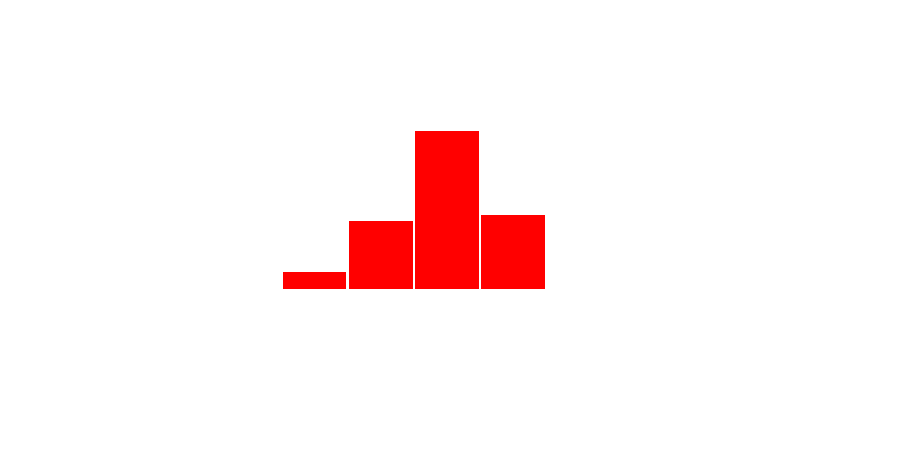
\includegraphics[scale = 0.1, clip = true, trim= 50px 60px 50px 60px]{hist-2b62bb5f7ccb31fe66208a895c8dd549.pdf} \\ 
  asserts\_per\_kloc & Number of assert statements per 1,000 lines of source code & 0.00 & 200.30 & 40.37 & 479.11 & 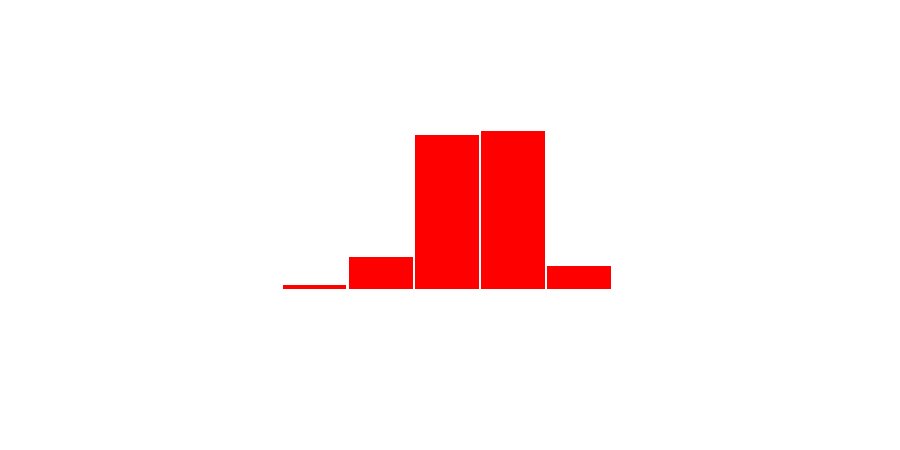
\includegraphics[scale = 0.1, clip = true, trim= 50px 60px 50px 60px]{hist-4ad84a89acf32483001ce11c881622b8.pdf} \\ 
  watchers & Project watchers (stars) at creation & 4.00 & 1,778 & 310.00 & 11,114 & 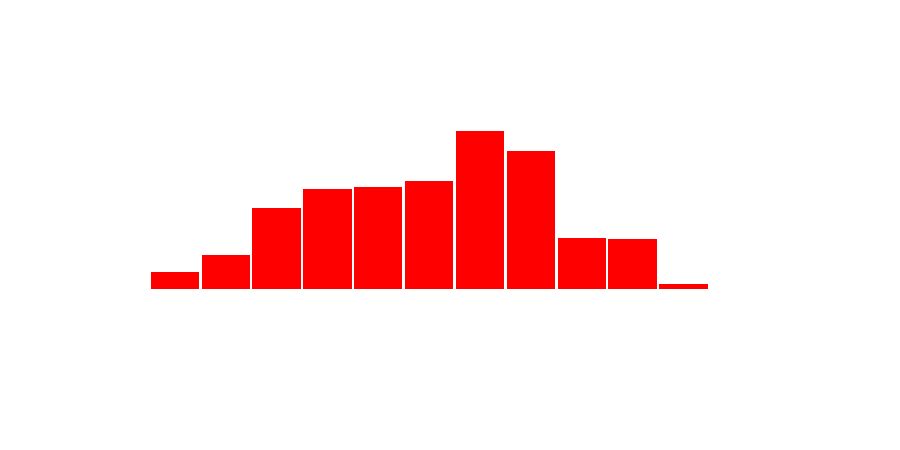
\includegraphics[scale = 0.1, clip = true, trim= 50px 60px 50px 60px]{hist-d097a7d1786ca9917e46e0fda1adb365.pdf} \\

  \multicolumn{2}{l}{\bf{Developer Characteristics}}\\
  
  prev\_pullreqs & Number of pull requests submitted by a specific developer, prior to the examined one & 0.00 & 42.81 & 11.00 & 196.00 & 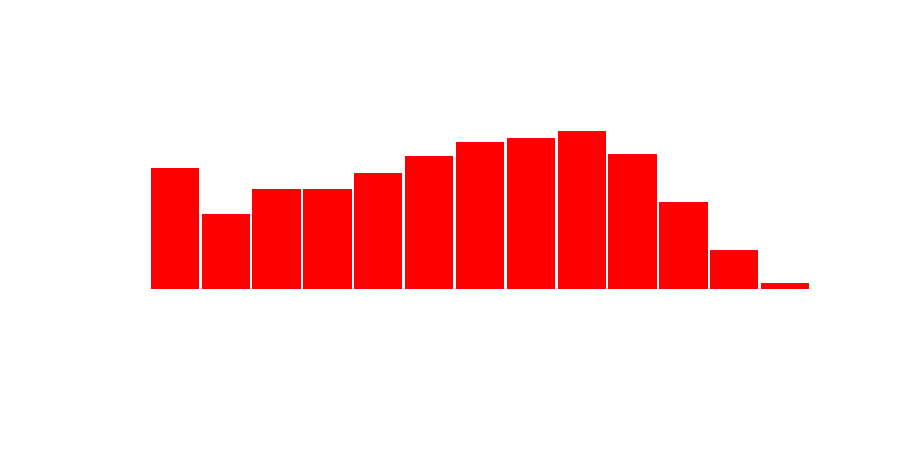
\includegraphics[scale = 0.1, clip = true, trim= 50px 60px 50px 60px]{hist-a2f7f60851dfa13cfbe0227d1d233767.pdf} \\ 
  requester\_succ\_rate & The percentage of the developer's pull requests that have been merged up to the creation of the examined one & 0.00 & 0.51 & 0.62 & 1.00 & 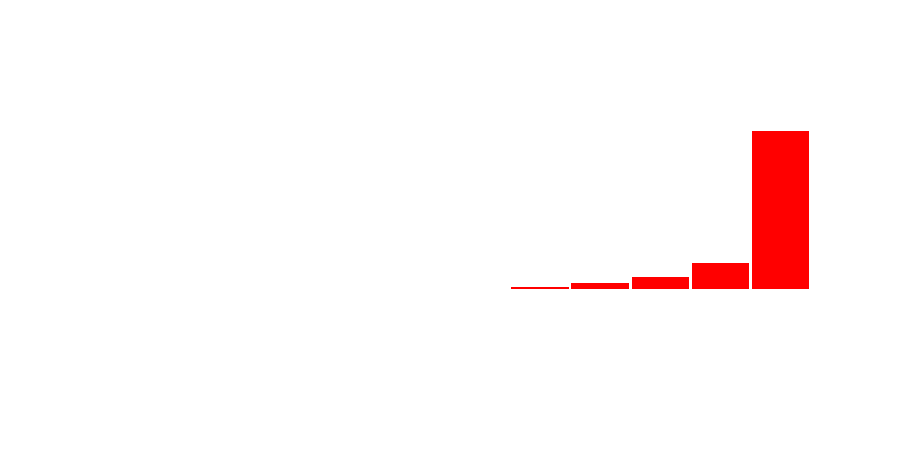
\includegraphics[scale = 0.1, clip = true, trim= 50px 60px 50px 60px]{hist-9363017165c3ded62457750f1c67c1af.pdf} \\ 
  followers & Followers to the developer at creation & 0.00 & 20.93 & 4.00 & 80.00 & 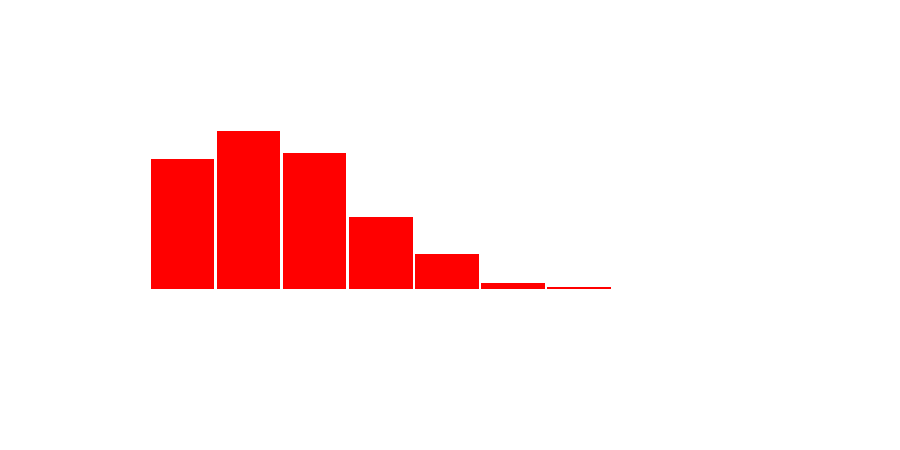
\includegraphics[scale = 0.1, clip = true, trim= 50px 60px 50px 60px]{hist-a7f2f738f15a09420e70e9a2c30e2aef.pdf} \\ 
   \hline
\end{tabular}
\caption{Selected features and descriptive statistics. A data point is a pull request. Historgrams are in log scale.} 
\label{tab:features}
\end{table*}


\begin{figure}
  \begin{center}
    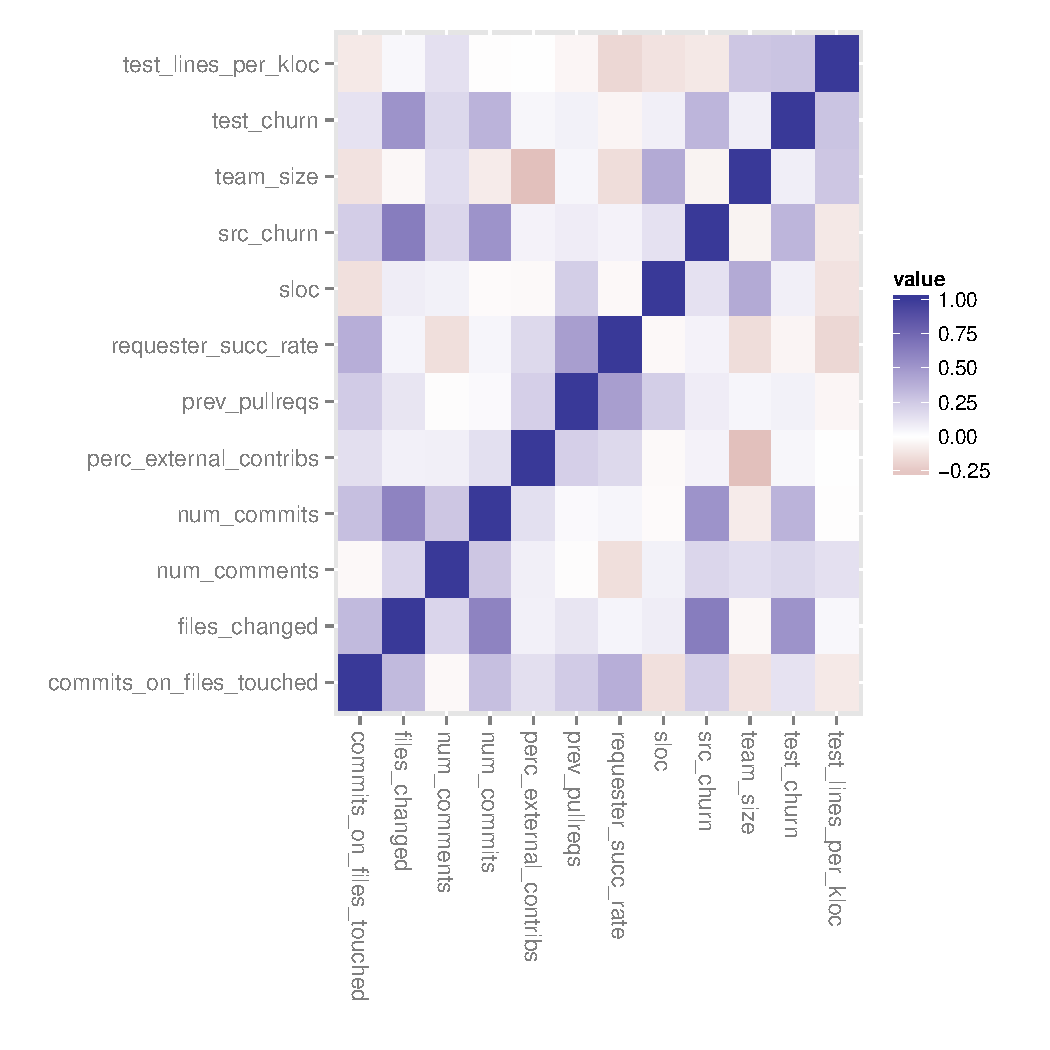
\includegraphics[scale=0.5]{cross-cor-heat.pdf}
  \end{center}
  \caption{Cross correlation heat map (Spearman) for selected features.}
  \label{fig:crosscor}
\end{figure}

\subsection{Qualitative data}
\label{sec:qualitative}
To investigate how pull requests are used in practice and why some pull requests
are not merged, we performed in-depth examination of random samples of pull
requests followed by coding and thematic analysis. 

%To examine how pull requests are used in practice, we categorized
%100 randomly selected pull requests, sampled from the dataset described above,
%in two categories: patches and feature discussions. We drew those categories
%from our experience as pull request users and also by consulting 
%the interviews in Pham et al.~\cite{Pham13} and Marlow et al.~\cite{Marlo13}.

To discover the reasons for pull request rejection, we again randomly sampled
cases from our pull request project dataset. 100 pull requests were initially
used by the first coder to identify discrete reasons for closing pull requests
(bootstrapping sample), while a different set of 100 pull requests were used by
all three coders to validate the identified categories (cross-validation
sample). After cross validation, a further 150 randomly selected pull requests
were added to the bootstrapping sample to construct the finally analyzed
dataset.

\section{Popularity of Pull-based Development}
\label{sec:github}
% latex table generated in R 2.15.3 by xtable 1.7-1 package
% Fri Sep  6 17:15:25 2013
\begin{table*}[ht]
\centering
\begin{tabular}{rccccccc}
  \hline
description & min & quant\_5 & median & mean & quant\_95 & max & histogram \\ 
  \hline
Number of participants & 0.00 & 0.00 & 1.00 & 1.39 & 3.00 & 91.00 & 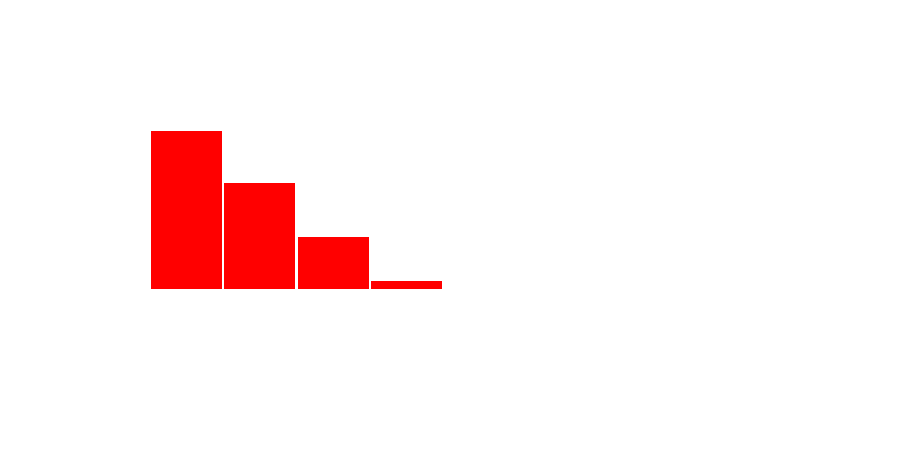
\includegraphics[scale = 0.1, clip = true, trim= 50px 60px 50px 60px]{hist-c83eb37a528ffcd758150a237ae378c7.pdf} \\ 
  Number of comments & 0.00 & 0.00 & 0.00 & 1.70 & 7.00 & 642.00 & 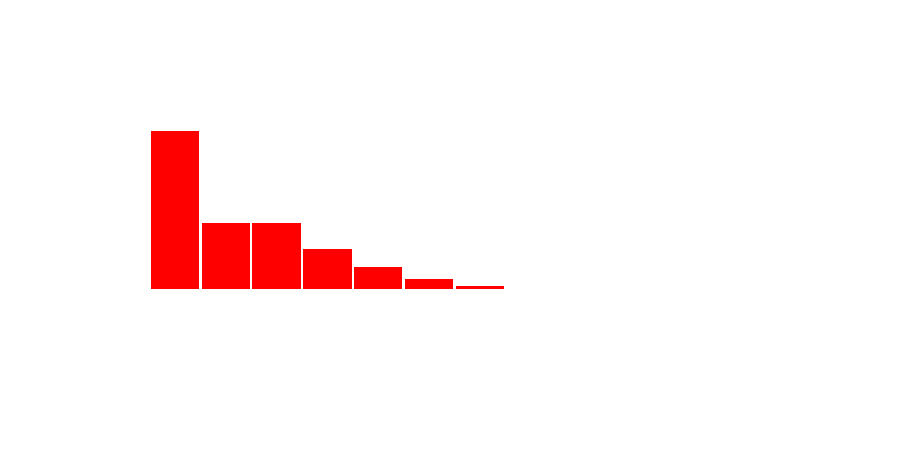
\includegraphics[scale = 0.1, clip = true, trim= 50px 60px 50px 60px]{hist-0d7111a5679c9d7ae097710bfbe5ad46.pdf} \\ 
  Number of commits & 1.00 & 1.00 & 1.00 & 5.00 & 14.00 & 1745.00 & 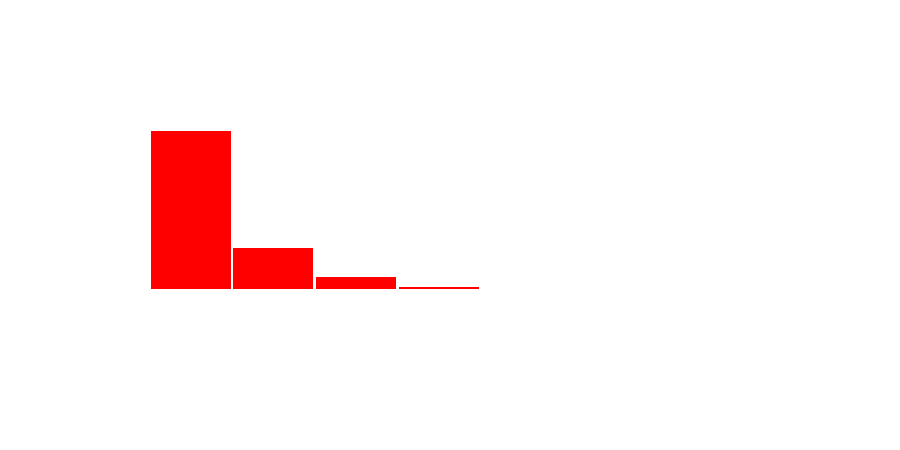
\includegraphics[scale = 0.1, clip = true, trim= 50px 60px 50px 60px]{hist-a86184e179390a51b3bf0b4a000ff1bf.pdf} \\ 
  Time to merge (min) & 0.00 & 0.00 & 157.00 & 7315.10 & 28883.30 & 1493913.00 & 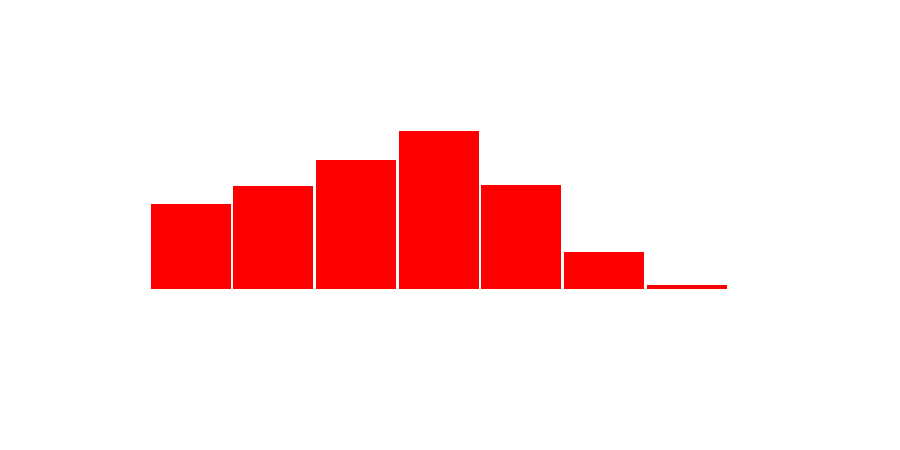
\includegraphics[scale = 0.1, clip = true, trim= 50px 60px 50px 60px]{hist-d5b282b6f57817578bf430989f92d122.pdf} \\ 
  Time to close (min) & 0.00 & 0.00 & 1108.00 & 30302.73 & 172754.95 & 1556363.00 & 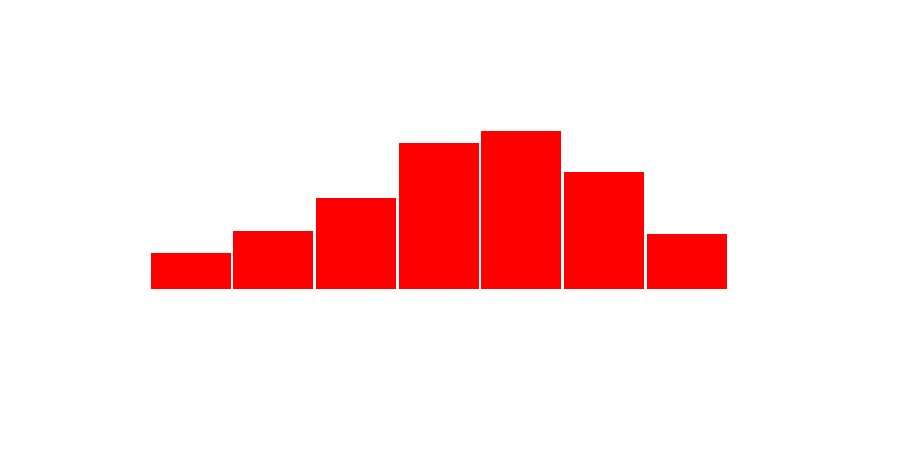
\includegraphics[scale = 0.1, clip = true, trim= 50px 60px 50px 60px]{hist-b2793dce9a27260faa7c8b85aeb789d2.pdf} \\ 
   \hline
\end{tabular}
\caption{Descriptive statistics for pull requests across all projects in the GHTorrent dataset (1.8M). Historgrams are in log scale.} 
\label{tab.overall.stats}
\end{table*}


Github is a very popular development site. As of August 2013, Github reports
more than 7 million repositories and 4 million users. However, not all those
projects are active: in the period Feb 2012 --- Aug 2013, the {\sc ght}orrent dataset captured events initiated by
(approximately) 2,281,000 users affecting 4,887,500 repositories. The majority
of registered repositories are forks of other repositories, special repositories
hosting user web pages (named as \texttt{<name>.github.com}), program
configuration files (\texttt{dotfiles}) and temporary repositories for
evaluating Git (\texttt{try\_git}). In the {\sc ght}orrent dataset, less than half
(1,877,660 or 45\%) of the active repositories are original repositories. From
those, 587,800 (or 28\% in total) received a commit in 2012.

Pull requests are enabled by default on all repositories opened on Github. On a
monthly basis, the average number of pull requests per repository is increasing
(Figure~\ref{fig:pullreq-per-month}). From the set of original repositories as
described above, 92,600 received at least one pull request in 2013. During the
same period, 898,550 original repositories used the shared repository approach,
having received commits by more than one developers and no pull requests. The
situation is similar during the first eight months of 2013; 42,400 repositories
received a pull request while 222,967 used the shared repository approach
exclusively. While pull request usage is increasing overall, they are not the
most popular approach for distributed software development yet.

An overview
For those projects that received pull requests in 2013, the mean number of pull
requests per project is relatively low at 7.1 (percentiles: 5\%: 1, 95\%: 21);
however, the distribution of the number of pull requests in projects is highly skewed.
From the pull requests that have been opened in 2012, 73,07\% have been merged
using Github facilities,
thereby indicating that pull requests in principle can work as a medium for
obtaining external contributions. Moreover, even though one might expect that it
is the well known projects that receive most pull requests, this is moderately supported by our data: the Spearman rank correlation between the number of
watchers of a project and the number of pull requests it has received is $\rho = 0.36$ ($p < 0.001, n = 235,564$).

\begin{figure}[t]
  \centering
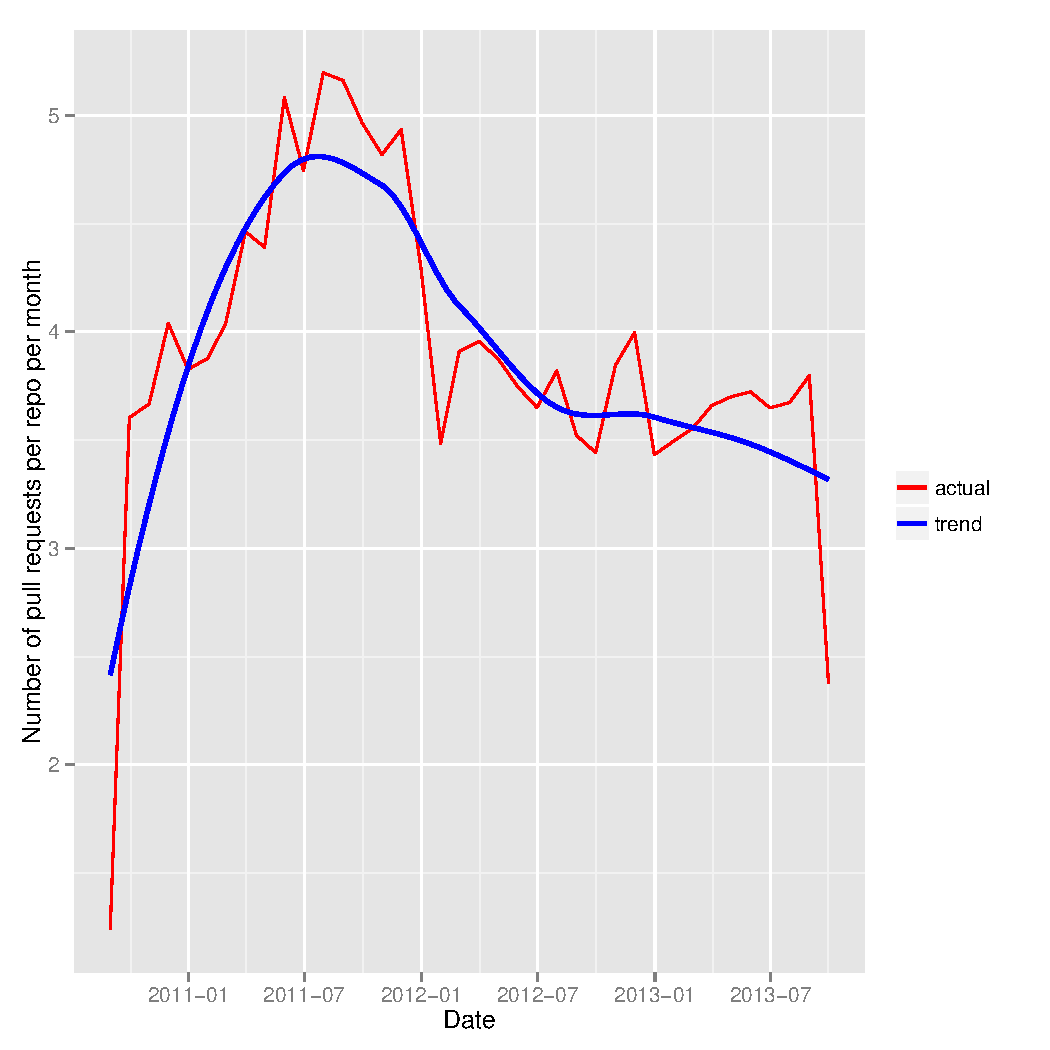
\includegraphics[scale=0.35]{num-pullreqs-month}
\label{fig:pullreq-per-month}
\caption{Pull requests on Github}
\end{figure}


Reviews on a pull request can either target the pull as whole or the individual commits,
thereby resembling a code review. 
Even though any Github user can participate to the
review process, usually it is the project community members that do so:
only 0.011\% of pull request comments come from users that have not
committed to the project repository.
Pull requests receive comments quite frequently: on average, each pull
request receives 12 (quantiles: 5\%: 2, 95\%: 35) discussion comments.

Issues and pull requests are dual on Github; for each pull request, an issue is
opened automatically. Commits can also be attached to issues to convert them to
pull requests (albeit with external tools). This duality enables project
administrators to treat pull requests as work items, which can be managed using
the same facilities used for issues. Across projects that received pull
requests in 2012, 35\% also received a bug report (not pull-request based) 
on the Github issue tracker, indicating a strong use of Github's collaboration
facilities by both the project and the project community.

%Pull requests in their current form were introduced by Github in late August
%2010. As can be seen in Figure~\ref{fig:before-after-pr}, on certain long lived
%projects, the introduction of pull requests had significantly increased the
%number of contributors per month. To investigate whether the introduction of
%pull requests had a measurable effect on projects that used them, we calculated
%the mean number of active developers per month for a period of 12 months before
%and after the introduction of pull requests. We filtered out projects that begun
%using pull requests only after September 2011 and those whose average number of
%developers is less than two (indicating self-submission and acceptance of pull
%requests). We performed a paired Mann-Whitney test across the means for each
%project, which indicated a statistically significant difference ($n = 362, V =
%56690, p < 0.001$). We also calculated the effect size using Cliff's $\delta =
%0.42$. This indicates a statistically significant increase in the mean number of
%developers per month after the introduction of pull requests, even though this
%does not necessarily mean that pull requests are indeed the reason.
%
%\begin{figure}
%  \begin{center}
%    
\includegraphics[scale=0.5]{num-commiters-after-pr}
%  \end{center}
%  \caption{Number of committers before and after the introduction of pull
%  requests by Github. The lines are smoothed using the local polynomial
%  regression fitting method, to account for monthly fluctuations.}
%  \label{fig:before-after-pr}
%\end{figure}


\fbox{
\begin{minipage}{0.46\textwidth}
\emph{RQ1: 14\% of repositories are using pull requests on Github. Pull request usage is increasing, even though the proportion of
repositories using them is relatively stable.}
\end{minipage}}



%% latex table generated in R 2.15.3 by xtable 1.7-1 package
% Fri Aug 23 15:19:16 2013
\begin{table}[ht]
\centering
{\small
\begin{tabular}{rrrrrrrrrrrrr}
  \hline
 & team\_size & num\_commits & files\_changed & perc\_external\_contribs & sloc & src\_churn & test\_churn & commits\_on\_files\_touched & test\_lines\_per\_kloc & prev\_pullreqs & requester\_succ\_rate & num\_comments \\ 
  \hline
team\_size & 1.00 & -0.09 & -0.03 & -0.28 & 0.41 & -0.04 & 0.08 & -0.15 & 0.26 & 0.03 & -0.19 & 0.16 \\ 
  num\_commits & -0.09 & 1.00 & 0.57 & 0.14 & -0.00 & 0.50 & 0.32 & 0.28 & -0.02 & 0.02 & 0.04 & 0.26 \\ 
  files\_changed & -0.03 & 0.57 & 1.00 & 0.06 & 0.09 & 0.62 & 0.49 & 0.30 & 0.03 & 0.12 & 0.06 & 0.17 \\ 
  perc\_external\_contribs & -0.28 & 0.14 & 0.06 & 1.00 & -0.03 & 0.05 & 0.04 & 0.15 & 0.01 & 0.22 & 0.13 & 0.11 \\ 
  sloc & 0.41 & -0.00 & 0.09 & -0.03 & 1.00 & 0.16 & 0.06 & -0.14 & -0.15 & 0.21 & -0.02 & 0.04 \\ 
  src\_churn & -0.04 & 0.50 & 0.62 & 0.05 & 0.16 & 1.00 & 0.33 & 0.21 & -0.11 & 0.09 & 0.07 & 0.18 \\ 
  test\_churn & 0.08 & 0.32 & 0.49 & 0.04 & 0.06 & 0.33 & 1.00 & 0.12 & 0.31 & 0.06 & -0.02 & 0.16 \\ 
  commits\_on\_files\_touched & -0.15 & 0.28 & 0.30 & 0.15 & -0.14 & 0.21 & 0.12 & 1.00 & -0.08 & 0.25 & 0.34 & -0.00 \\ 
  test\_lines\_per\_kloc & 0.26 & -0.02 & 0.03 & 0.01 & -0.15 & -0.11 & 0.31 & -0.08 & 1.00 & -0.03 & -0.12 & 0.14 \\ 
  prev\_pullreqs & 0.03 & 0.02 & 0.12 & 0.22 & 0.21 & 0.09 & 0.06 & 0.25 & -0.03 & 1.00 & 0.47 & -0.02 \\ 
  requester\_succ\_rate & -0.19 & 0.04 & 0.06 & 0.13 & -0.02 & 0.07 & -0.02 & 0.34 & -0.12 & 0.47 & 1.00 & -0.10 \\ 
  num\_comments & 0.16 & 0.26 & 0.17 & 0.11 & 0.04 & 0.18 & 0.16 & -0.00 & 0.14 & -0.02 & -0.10 & 1.00 \\ 
   \hline
\end{tabular}
}
\caption{Cross correlation matrix (Spearman) between examined factors} 
\label{tab:crosscor}
\end{table}


\section{Pull Request Lifecycle Characteristics}
\label{sec:pullreqchar}

\textbf{Lifetime of pull requests.}
After being submitted, pull requests can be in two states: merged or closed
(and therefore not-merged).
In our dataset, most pull requests (mean: 84.73\%) are getting
merged. This result is higher than the overall we calculated for
Github, but this can be attributed to the fact that the dataset generation
process employs heuristics to detect merges outside Github.

For merged pull requests, an important property is the time required to process
and merge them. The time to merge distribution is highly skewed, with the great
majority of merges happening very fast. Measured in days, 95\% of the pull
requests are merged in 26, 90\% in 10 and 80\% in only 3.7 days. An interesting
observation is that there are many (43,557 or 30\% of our sample) pull requests
which are merged in under one hour; the majority of such pull requests (60\%)
come from the community, while their source code churn is significantly
lower than that of the remaining pull requests (medians: 5 and 13 respectively). If we compare the time to
process pull requests that are being merged against those that are not, we can
see (Figure~\ref{fig:close-merged-unmerged}) that pull requests that have been
merged are closed much faster (median: 434 minutes) than unmerged (median: 2250
minutes) pull requests.
The results of an unpaired Mann-Witney test ($p < 0.001$) showed that this difference is statistically significant, with a relatively
significant effect size (Cliff's $\delta: 0.32$). This means that pull requests
are either processed fast or left lingering for long before they are closed.

Based on these observations, a question that emerges is
whether the pull requests originating from main team members are treated faster
than those from external contributors. To answer it, we performed an unpaired
Mann-Witney test among the times to merge pull requests from each group. The
result is that while the two groups differ in a statistically significant manner
($n_1 = 51,829, n_2 = 89,454, p < 0.001$), the apparent difference is negligible
(Cliff's $\delta: -0.09$, see also Figure~\ref{fig:lifetime-boxplot}). This
means that merged pull requests received no special treatment, irrespective
whether they came from core team members or from the community.

On a per project basis, if we calculate the mean time to merge a pull request,
we see that in the majority of projects (65\%), the mean time to merge a pull
request is less than 7 days. The mean time to merge a pull request per project
is not correlated with the project's size, as indicated by a low Spearman
correlation value ($\rho = -0.05$) nor the project's test coverage ($\rho =
0.27$). It is however, strongly correlated ($\rho = -0.69$) with the pull
request initiator's track record: the highest the number of pull requests a
developer has submitted to the same project, the lowest the time to process it.
Moreover, projects are not getting faster at pull request processing by
processing more pull requests; the correlation between the average time to merge
and the number of pull requests is weak ($\rho = -0.23, n = 291, p < 0.01$).

\fbox{
\begin{minipage}{0.46\textwidth}
\emph{80\% of pull requests are merged in less than 3 days, while 30\% are
merged within one hour. Pull requests are treated the same irrespective of
their origin (project team or community). The developer's track record
is an indicator of how fast a pull request will be merged.}
\end{minipage}}

\begin{figure}
\centering
%\subfigure[Percentage of pull requests that have been merged per project.
%Project names are omitted for clarity.]{
%  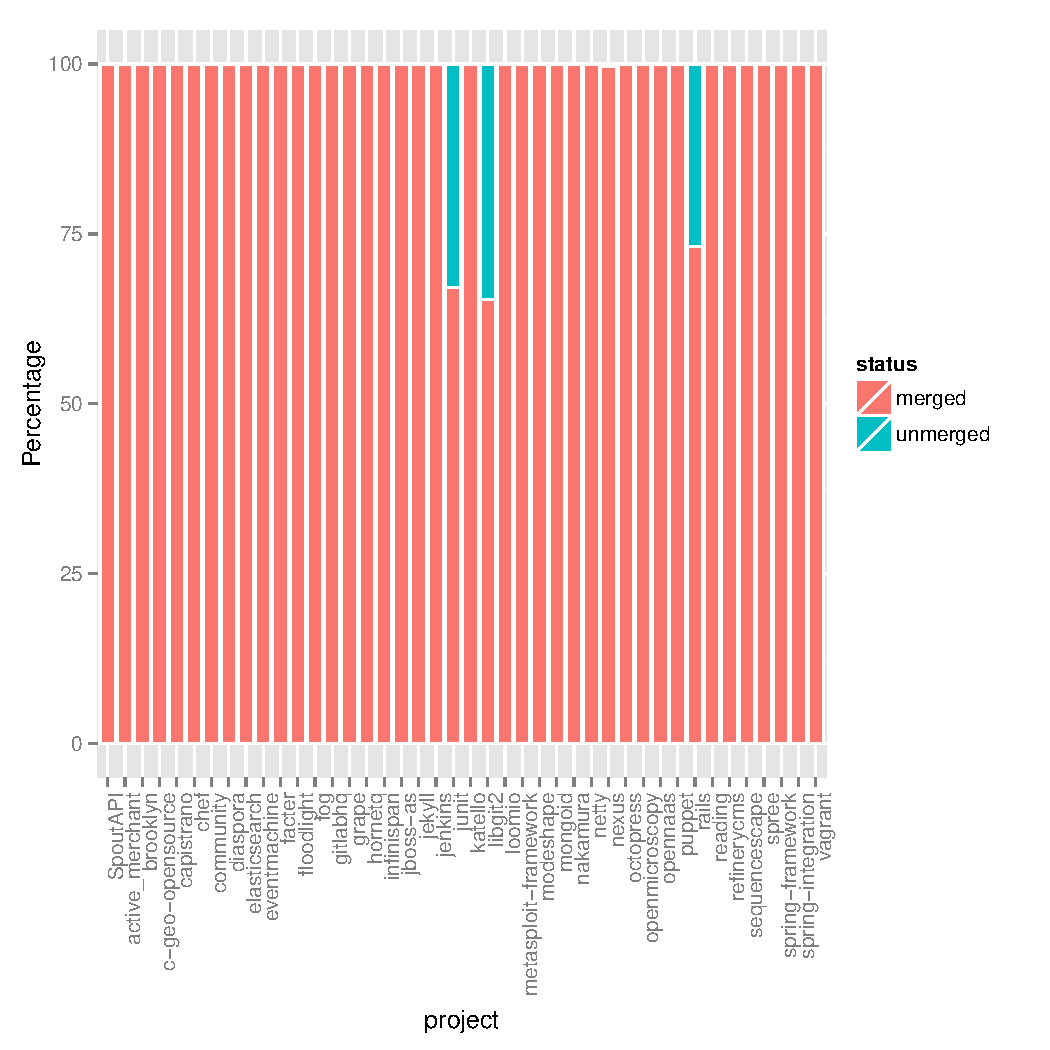
\includegraphics[scale=0.35]{perc-merged.pdf} 
%  \label{fig:perc-merged}
%}
%\subfigure[Time to merge pull requests.]{
%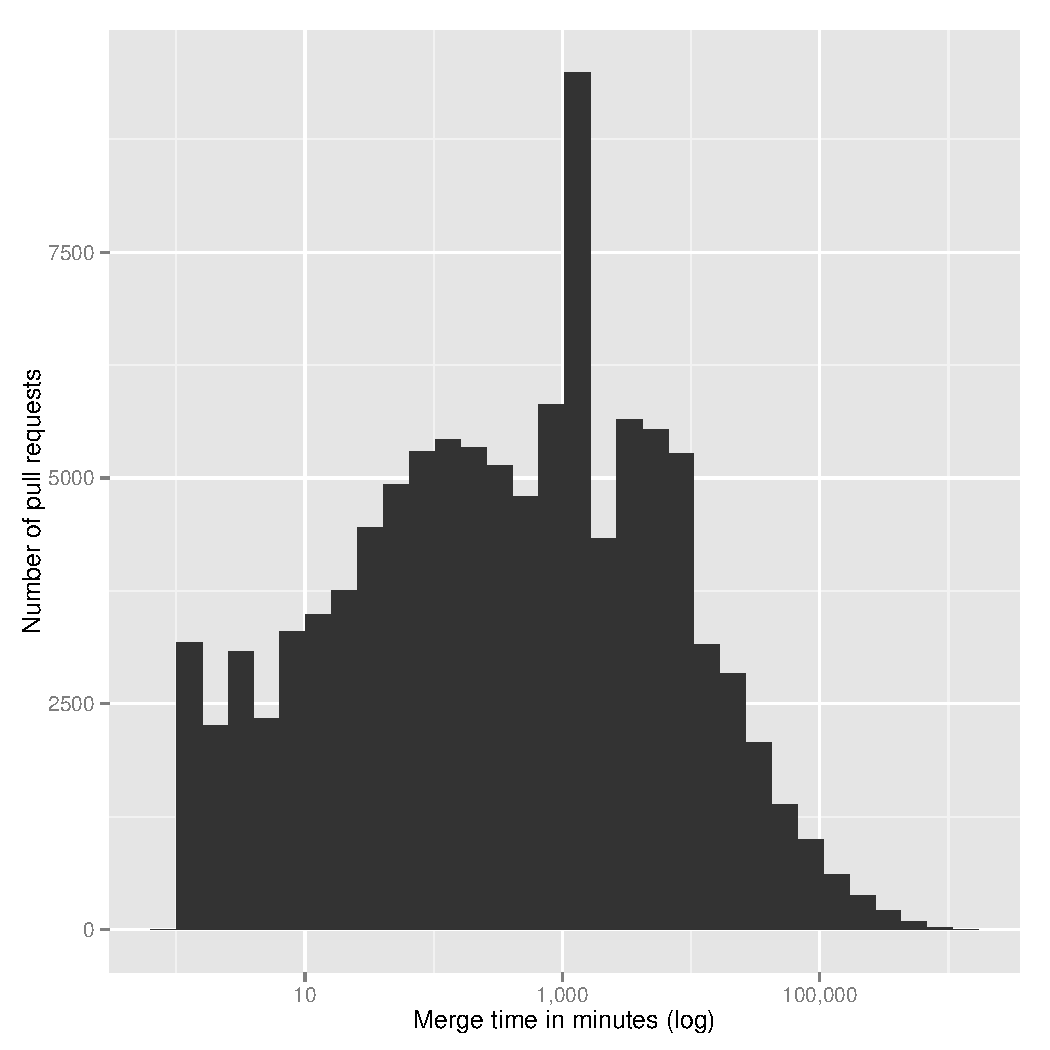
\includegraphics[scale=0.3]{pr-lifetime-hist.pdf}
%\label{fig:pull-req-merge-time}
%}
\subfigure[Time to close pull requests.]{
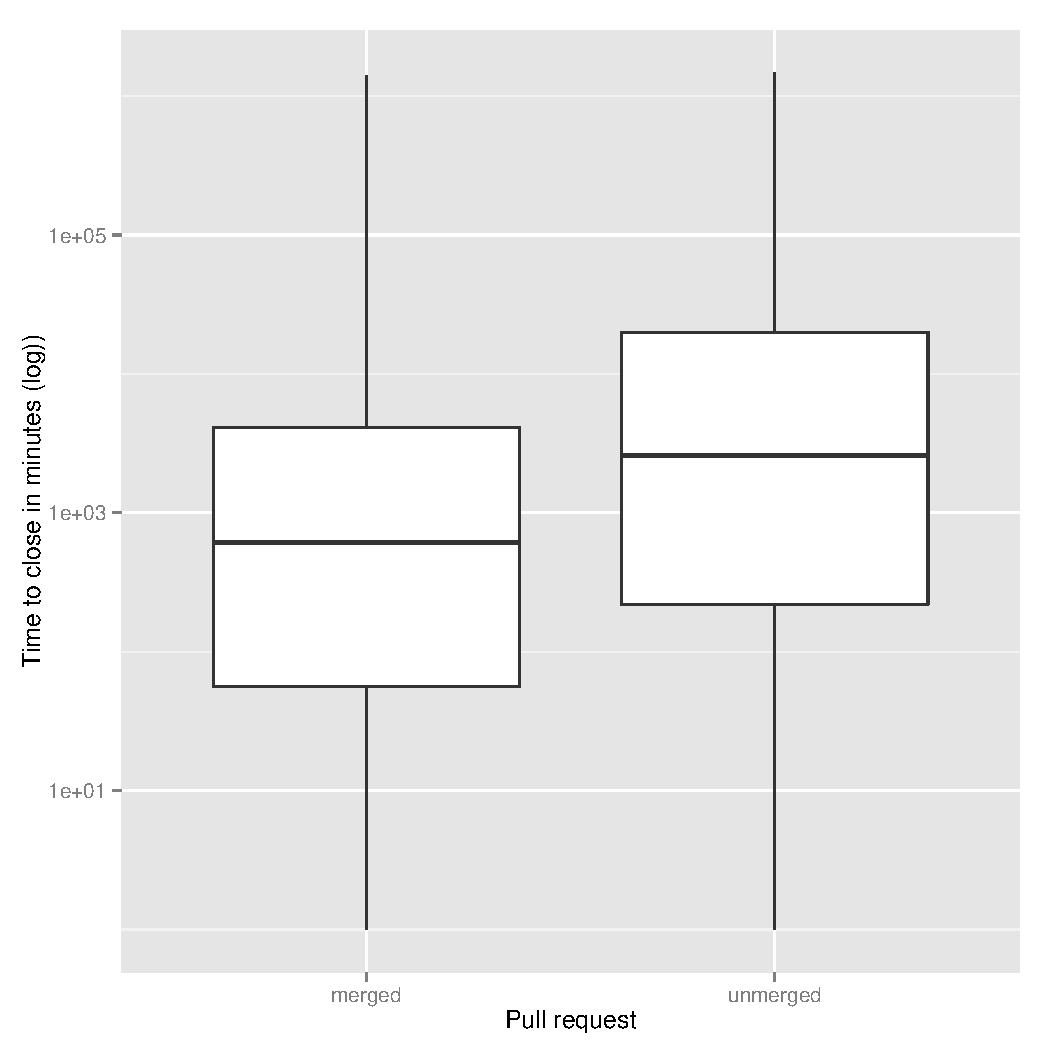
\includegraphics[scale=0.35]{close-merged-unmerged.pdf}
\label{fig:close-merged-unmerged}
}
\subfigure[Time to merge pull requests for internal vs external team members.]{
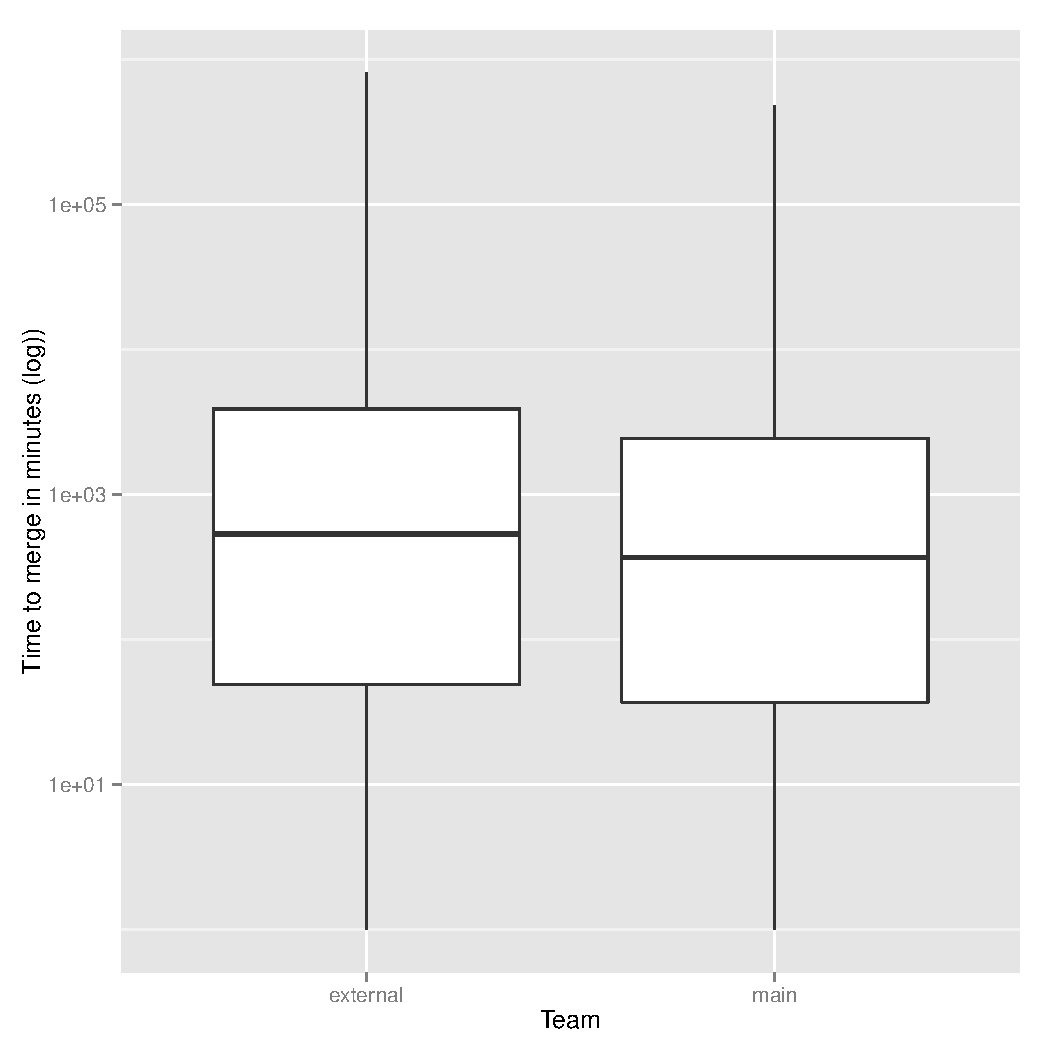
\includegraphics[scale=0.35]{merge-internal-external.pdf}
\label{fig:lifetime-boxplot}
}
%\subfigure[Size of pull request patch.]{
%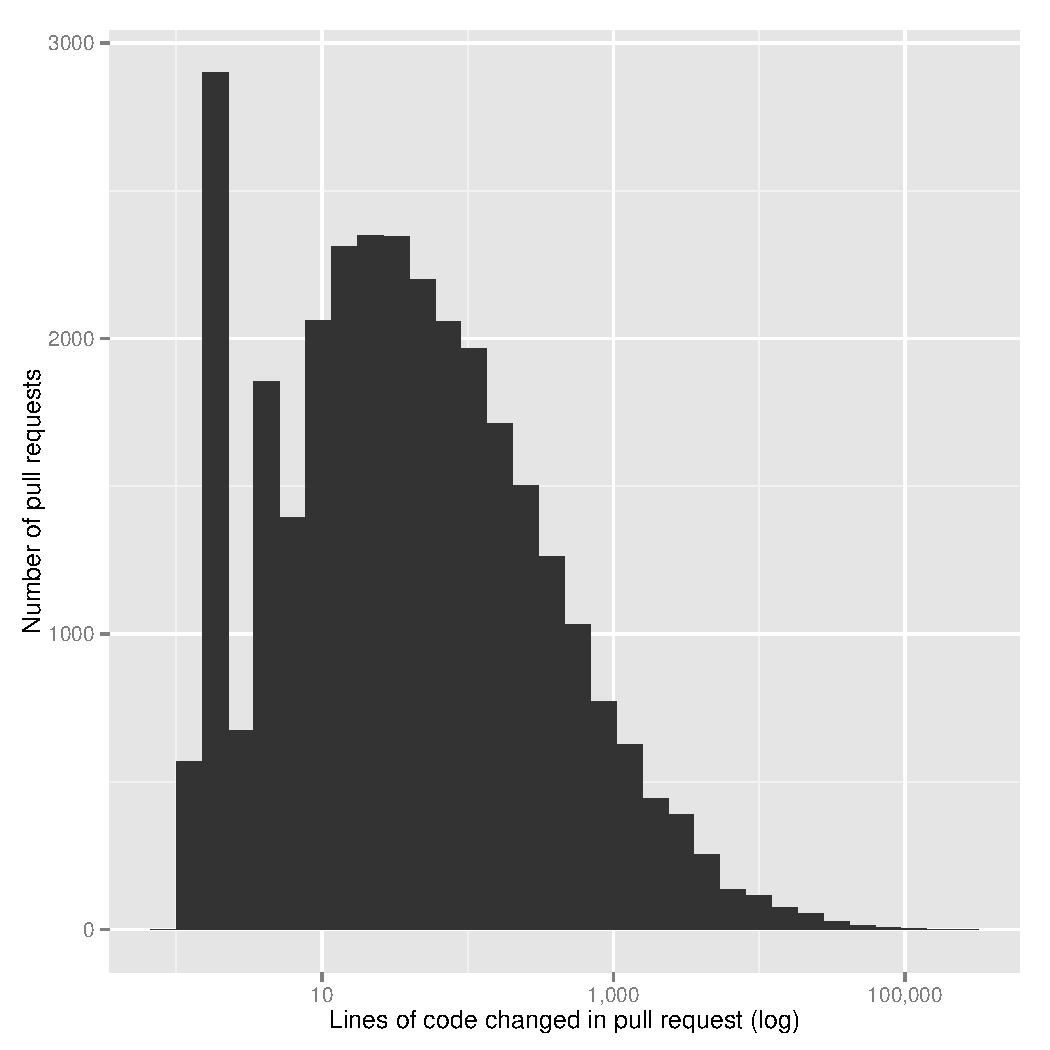
\includegraphics[scale=0.3]{pr-size-hist.pdf}
%\label{fig:pull-req-patch}
%}
%\subfigure[Number of files changed by pull request.]{
%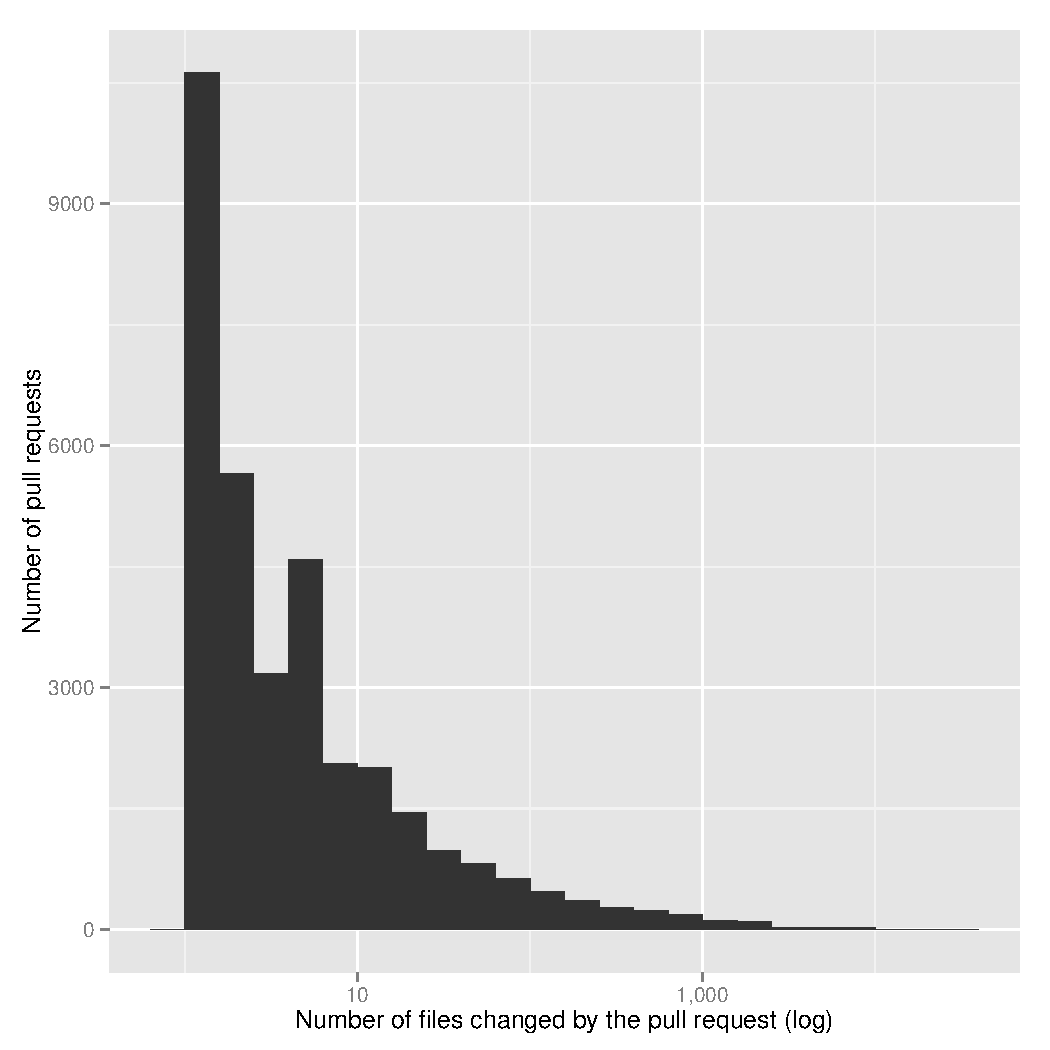
\includegraphics[scale=0.3]{pr-size-files-changed-hist.pdf}
%\label{fig:pull-req-files}
%}
\subfigure[Percentage of external commenters and comments per project. Bars
are sorted by percentage of external commenters. Project names omitted for
clarity.]{
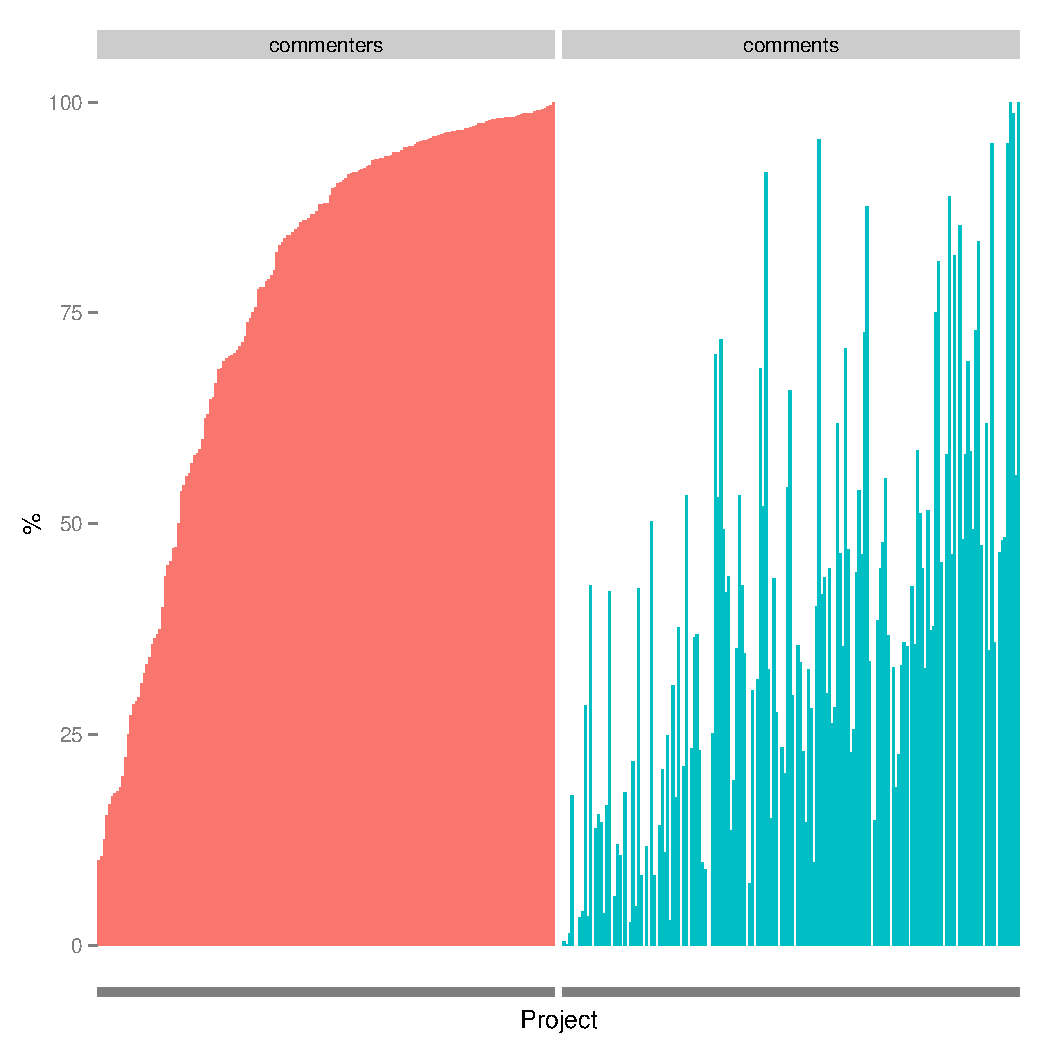
\includegraphics[scale=0.35]{perc-external-commenters-comments.pdf}
\label{fig:pull-num-comments}
}
\caption{Dataset characteristics.}
\end{figure}

\textbf{Sizes of pull requests.}

A pull request bundles together a set of commits; the number of commits on a
pull request is generally less than 10 (95\% percentile: 11, 90\% percentile: 6,
80\% percentile: 3), with a median of 1. The number of files that are changed by
a pull request is generally less than 20 (95\% percentile: 36, 90\% percentile:
17, 80\% percentile: 7), with median number of 2. The number of total lines
changed by pull requests is on average less than 500 (95\% percentile: 1227,
90\% percentile: 497, 80\% percentile: 168) with a median number of 20.

Except from the project's source code, pull requests also modify test code. In
our sample, 33\% of the pull requests included modifications in test code, while
4\% modified test code exclusively. Of the pull requests that included tests,
72\% were merged, which is similar to the average. The presence of tests in a
pull request does not seem to affect the merge time either: an unpaired
Mann-Witney test shows that while there is a difference in the means of the pull
request merge time for pull requests that include tests ($tests = 8831, no\_tests
= 19061, p < 0.001$), the effect size is very small ($\delta = 0.07$). This
result contradicts the findings by Pham et al.~\cite{Pham13}, where
interviewed developers identified the presence of tests as a major factor for
the acceptance of pull requests.

\fbox{
\begin{minipage}{0.46\textwidth}
\emph{Including test code does not help pull requests to be processed faster.}
\end{minipage}}


\textbf{Discussion and code review.}
Once a pull request has been submitted, it is open for discussion until
it is merged or closed. The discussion is usually brief: 95\% of pull
requests receive 10 comments or less (80\% less than 4 comments). 
The number of comments in the discussion is neither correlated with
whether a pull request will be merged nor with the life time of the
pull request.

Any Github user can participate to the discussion of any pull request. Usually,
the discussion occurs between core team members trying to understand the changes
introduced by the pull request and community members (often, the pull
request creator) that explain it. Figure~\ref{fig:pull-num-comments} presents
the distribution of external commenters and comments to pull request discussion
across projects in our samples. We observe that in most projects, more than half
of the commenters are community members. This is not true however for the number
of comments; in most projects the majority of the comments come from core team
members. One might think that the bigger the percentage of external commenters
on pull requests the more open the project is and therefore the highest the
percentage of external contributions; a Spearman correlation test quickly
indicates that this is not true ($\rho = 0.22, n = 88, p < 0.05$).

\section{Results}
\label{sec:accrej}

\begin{table}
  \centering
  \begin{tabular}{lcccc}
    \hline
    {\bf classifier} & {\sc auc} & {\sc acc} & {\sc prec} & {\sc rec} \\
    \hline
    \multicolumn{4}{l}{\textsf{mergedecision} task($n = 37,492$)} \\
    binlogregr    & 0.73 & 0.63 & 0.87 & 0.58  \\
    naivebayes    & 0.69 & 0.61 & 0.85 & 0.57  \\
    randomforest  & 0.94 & 0.87 & 0.93 & 0.93  \\
    svm           & 0.52 & 0.48 & 0.72 & 0.48  \\
    \hline
    \multicolumn{4}{l}{\textsf{merge time} task($n = 27,892$)} \\
    binlogregr    & 0.60 & 0.55 & 0.56 & 0.57  \\
    naivebayes    & 0.58 & 0.54 & 0.54 & 0.57  \\
    randomforest  & 0.73 & 0.61 & 0.65 & 0.70  \\
    svm           & 0.54 & 0.49 & 0.45 & 0.45  \\
    \hline
  \end{tabular}
  \caption{Classifier performance for the merge decision and merge time
  classification tasks. The results are means of 10-fold random selection
  cross validation (sample size 10,000), with 90\% train and 10\% test data.}
  \label{tab:classif-perf}
\end{table}

We run the classification processes according to the protocol specified in 
Section~\ref{sec:expprocess}. The data comprises of 
37,492 and 27,892 pull requests for the \textsf{merge decision} and \textsf{merge time}
classification task, respectively.
Based on the results presented in Table~\ref{tab:classif-perf},
we selected the \texttt{randomforest} classification algorithm for
both our experiments. For the \textsf{mergetime} experiment, \texttt{randomforest}
achieved an {\sc auc} of 0.73, with a prior probability of 50\%. For 
the \textsf{mergedecision} experiment, the prior probability was 74\% which
allowed the algorithm to achieve near perfect scores. In both cases,
the stability of the {\sc auc} metric across folds was good 
(\textsf{mergetime}: $\sigma_{auc} = 0.019$, \textsf{mergedecision}: $\sigma_{auc} = 0.008$).
%
%\begin{figure*}
%\centering
%\subfigure {
%  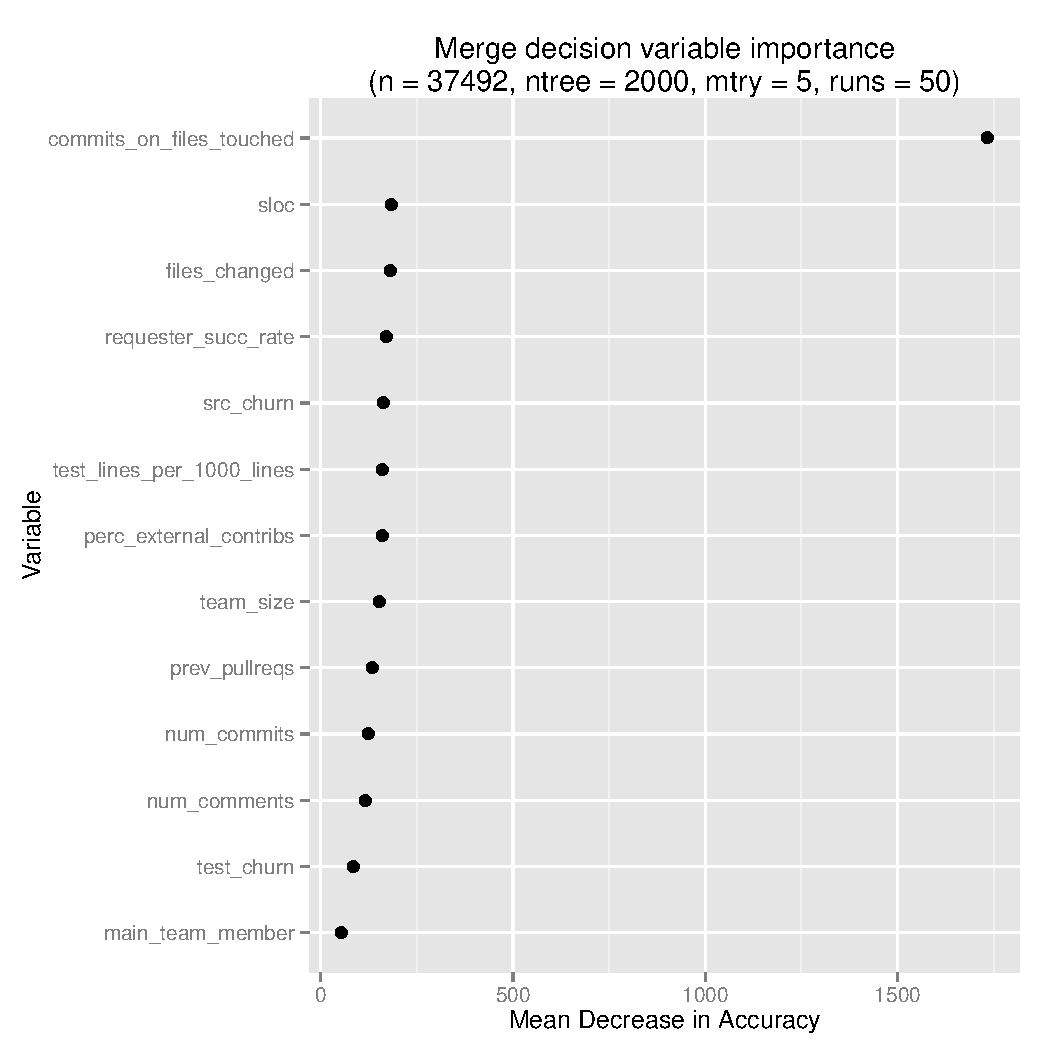
\includegraphics[scale=0.4]{varimp-merge-decision-37492-50.pdf} 
%  \label{fig:varimp-merge-decision}
%}
%\subfigure{
%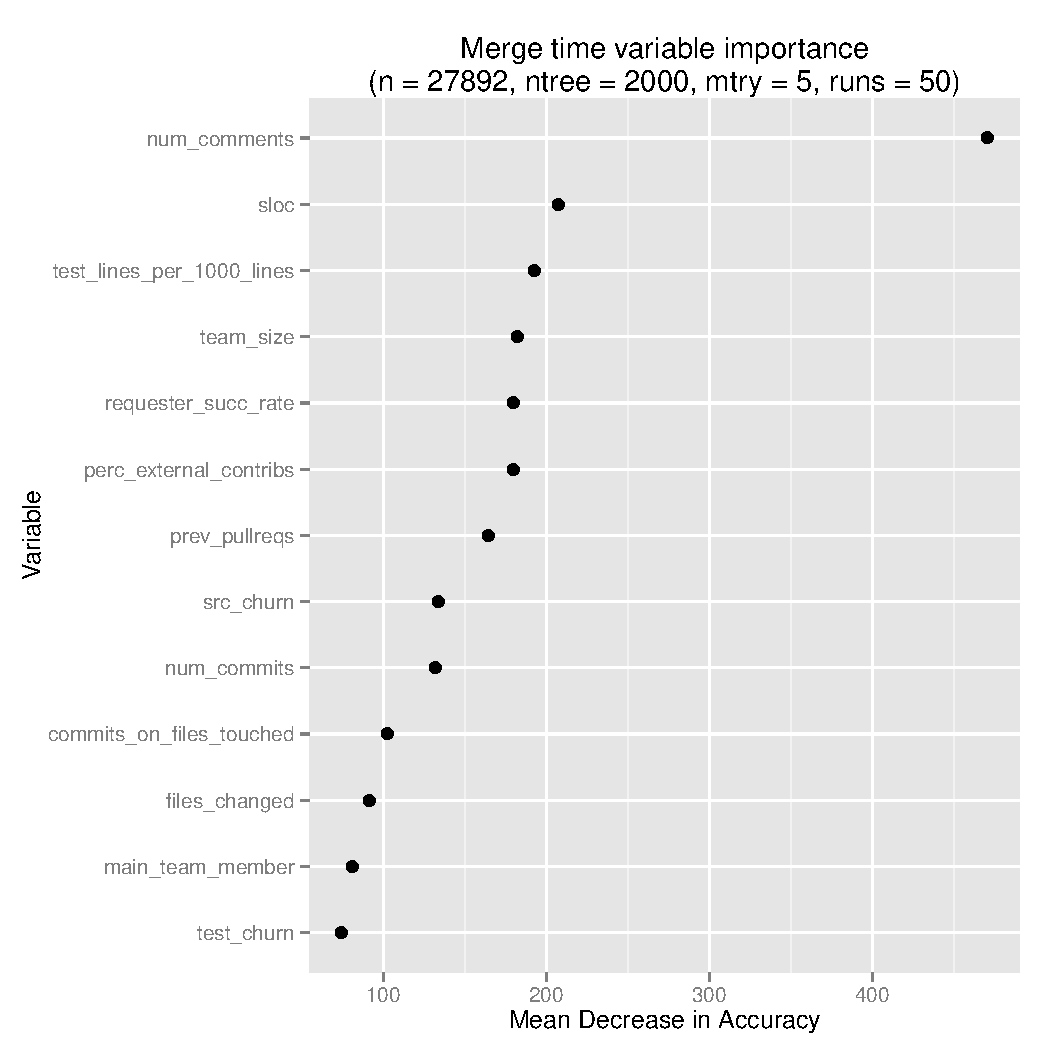
\includegraphics[scale=0.4]{varimp-merge-time-27892-50.pdf}
%  \label{fig:varimp-merge-time}
%}
%%\subfigure{
%%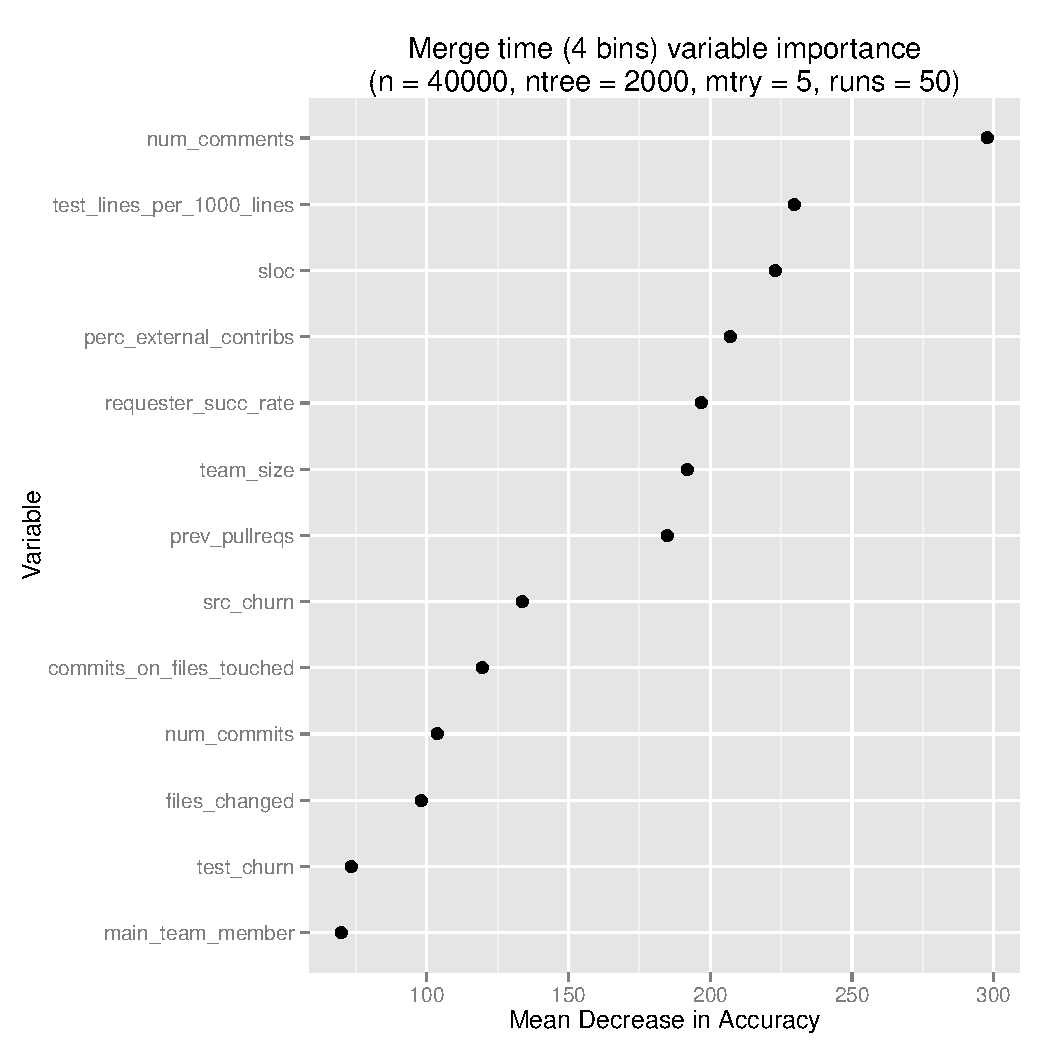
\includegraphics[scale=0.3]{varimp-merge-time-(4-bins)-40000-50.pdf}
%%  \label{fig:varimp-merge-time}
%%}
%\caption{Random forest feature importance for predicting merge decision (a) and merge time (b)}
%\label{fig:varimp}
%\end{figure*}

To extract the features that are important for each classification task, we
used the process suggested in reference~\cite{Genue10}. Specifically, we run
the algorithm 50 times on the full dataset for each experiment, using a large
number of generated trees (2000) and trying 5 random variables per split. We
then used the mean across 50 runs of the  Mean Decrease in Accuracy metric, as
reported by the {\sc r} implementation of the random forest algorithm, to
evaluate the importance of each feature. The results can be seen in
Figure~\ref{fig:varimp}.

Finally, to validate our feature selection, we rerun the 10-fold
cross-validation process with increasing number of predictor features starting
from the most important one per case.
In each iteration step, we add to the model the next most important feature.
We stop the process when the mean {\sc
auc} metric is within 2\% from the value in Table~\ref{tab:classif-perf} for
each task. The selected set of features should then be enough to predict the
classification outcome with reasonable accuracy, and therefore can be described
as important.

For the \textsf{mergedecision} task, the feature importance result is dominated
by the \texttt{commits\_\-on\_\-files\_\-touched} feature. By re-running the cross
validation process, we conclude that it suffices to use the features
 \texttt{commits\_\-on\_\-files\_\-touched}, \texttt{sloc} and \texttt{files\_changed}
to predict whether a pull request will be merged ({\sc auc:} 0.93, {\sc acc}:
0.86). Therefore, we can conclude that the decision to merge a pull request is
affected by whether it touches an actively developed part of the system (a
variation of the ``yesterday's weather'' hypothesis), how large the project's
source code base is and how many files the pull request changes.

\fbox{
\begin{minipage}{0.46\textwidth}
\emph{RQ2: The three main factors that affect the decision to merge a pull request are: i)
How active the area affect by the pull request has been recently ii) The size of the project iii) The number of files changed by the pull request.}
\end{minipage}}

For the \textsf{mergetime} task there is again a dominating feature, but the
difference is not as pronounced as in the previous case. However, if we re-run
the cross-validation process we see that the \texttt{num\_comments} along with
the \texttt{sloc} and the \texttt{test\_lines\_per\_1000\_lines} are enough to
enable \texttt{randomforest} to reach similar performance levels ({\sc auc:}
0.74, {\sc acc}: 0.65), as with the full feature set. From the results, we can
conclude that the discussion comments and the size of the project play a
significant role on how fast pull requests are processed. 

\fbox{
\begin{minipage}{0.46\textwidth}
\emph{RQ3: The three main factors that affect the time to merge a pull request
are: i) The number of discussion comments ii) The size of the project iii) The
project's test coverage.}
\end{minipage}}

\section{Discussion}
\label{sec:discussion}

\subsection{The pull-based development model}

\textbf{Development turnover.} One of the promises of the pull request model
is fast development turnover, i.e., the time between the submission of a pull
request and its acceptance in the project's main repository. In various studies of
the patch submission process in projects such as Apache and Mozilla, the
researchers found that the time to commit 50\% of the contributions to the main
project repository ranges from a few hours~\cite{Rigby08} to less than 3
days~\cite{Weiss08, Baysa12}. Our findings show that the majority (80\%) of
pull requests are merged within 3 days, while a very significant number (30\%)
are merged within one hour (independent of project size). These numbers are significantly faster indicating
that pull requests are more efficient than traditional email-based patches.
What's more important is that it is project-related factors that affect the
turnover time, rather than characteristics of the pull request. This means that
it is mostly up to the project to tune its processes (notably, reviewing and
testing) for faster turnover.

\fbox{
\begin{minipage}{0.46\textwidth}
\emph{Pull requests are faster to merge than email-based patches. Projects can
tune their reviewing and testing processes for faster turnover.}
\end{minipage}}

\textbf{Attracting contributions.}
Pham et al.~\cite{Pham13}, mention
that pull requests make casual contributions straightforward through
a mechanism often referred to as ``drive-by commits''. As the
relative cost to fork a repository is negligible on Github (54\% of the
repositories are forks), it is not uncommon for developers to fork other
repositories to perform casual commits, such as fixes to spelling mistakes or
indentation issues. In addition, Github provides web based editors
for various file formats, using which any user can edit a file in another
repository; Behind the scenes, Github will fork the repository and ask the user
to create a pull request to the original one. Such commits might be identified
as pull requests that contain a single commit from users that are not yet part
of the project's community. Even under this na\"ive definition, 7\% of pull
requests in 2012 can be classified as drive by commits. Moreover, 3.5\% of the
forks were created for the sole purpose of creating a drive-by commit. More
work needs to be done for the accurate definition and assessment of the
implications of drive-by commits, which we defer for future work.

\textbf{Crowd sourcing the code review.}
An important part of the contribution process to an open source project is the
review of the provided code. Rigby and German~\cite{Rigby06},
report that 80\% of the core team members are also participating in the code
reviews for patches, a number that is also in line with earlier findings by
Mockus et al.~\cite{MOCKU02}. In our dataset, we found that \emph{all} core
team members across all projects have participated in at least
one discussion in a pull request. Moreover, we found that in most projects
in our dataset, the community discussing pull requests is actually bigger
than the project team members, even though only in few cases does the community
contribute more to the discussion overall.

\fbox{
\begin{minipage}{0.46\textwidth}
\emph{Pull requests can help involve project community to the code review
process.}
\end{minipage}}

\textbf{Democratizing development.} One of the key findings of this work is
that pull requests are not treated differently based on their origin; both core
team members and external developers have equal chances to get their pull
request accepted within the same time boundaries. Indeed, even the
classification models we built assign to the corresponding feature the least
importance. In our opinion, this is a radical change in the way open source
development is being carried out. Before pull requests, most projects employed
membership promotion strategies~\cite{Jense07} to promote interested third party
developers to the core team. With pull requests, developers can contribute to
any repository, without loss of authorship information. The changes that those
contributions will get accepted are higher with pull requests; in our sample,
and also across Github, more than 70\% of external contributions are merged
(40\% in other studies~\cite{Rigby06, Weiss08}). Specialized sites such as
Ohloh and CoderWall track developer activity and help developers advertise their
expertise. We believe that the democratization of the development effort will
lead to a substantially stronger shared ecosystem; this remains to be
verified in further studies.

\subsection{Implications}

\textbf{Contributors.}
Prospective project contributors will want their
contributions to be accepted. Our research shows that pull requests that affect parts
of the project that  have been changed often lately (are ``hot'') are very
likely to get merged. Also, most pull requests that include test code are
accepted, while 80\% of the merged pull requests modify three or less files and include
patches less than 100 lines long. Therefore, our advice to contributors seeking
to add a particular feature or fix a bug is to ``keep it short''. If the contribution's purpose is to make the contributor known
to the project community, it is also beneficial to affect a project area that is
hot.

\textbf{Project Owners.} The primary job of the project owner, or owning team,
is to evaluate a list of pull requests and decide whether to apply them or not.
To make sure pull requests are processed on time, the obvious strategy would be
to enforce limits on the discussion as it does not seem to affect the decision
to merge a pull request significantly and only adds time overhead; however, this
may have adverse effects on the quality of the submitted contributions. A more
comprehensive strategy would include a clear articulation of what is expected
from a pull request, for example tests or localized changes, on a prominent
location in the project's Github page.\footnote{Surprisingly, a quick
investigation revealed that no project in our sample had such information in
the top-level {\sc readme}.md file.} Moreover, a project owner can invest in a
comprehensive test suite; this will improve the time to process a pull request,
especially if used with an automated continuous integration system.

% cd /cache && find . -type f -maxdepth 3|grep README.md|while read f; do if [ ! -z "`grep -i "pull request" $f`" ]; then echo $f; fi; done

%\textbf{Researchers.}
A direct application of our results is the construction of tools to help project owners to prioritize their work; since we can predict
with very high accuracy whether a pull request will be merged or not, a
potential tool might suggest which pull requests can be merged without further
examination by the time they arrive. Other tools might examine the quality of
the pull request at the contributor's site, and based on the base repository's
profile, would provide suggestions for improvement (e.g., more tests,
documentation). 

\subsection{Threats to validity}

\textbf{Internal validity.} Our statistical analysis uses random forests as a way
to identify and rank cross-factor importance on two response variables. While
this is a valid approach~\cite{Genue10}, we have yet to find other studies in
empirical software engineering that follow it. Moreover, the classification
scores in the \textsf{mergetime} case are not perfect, so feature ranking may
not be exactly the same given a different dataset. Further work is needed on
validating the models on data from different sources (e.g., manual pull
request handling in the Linux kernel) or projects in different languages. 

%\textbf{Internal validity.}
To analyze the projects, we extracted data from i) the {\sc ght}orrent relational
database ii) The {\sc ght}orrent raw database iii) each project's Git repository.
Differences in the data abstraction afforded by each data source may
lead to different results in the following cases: 
i) Cross-branch merges: {\sc ght}orrent currently does not record the source
    and target branch names that are affected by a pull request. Therefore, it
    is not possible to use the heuristics presented in
    Section~\ref{sec:expdata} to identify a merged branch, if the project
    does not use Github facilities to merge. In those cases, we
    report the pull request as non-merged. In our dataset, 810 (or 2\% in total)
    pull requests are label as non-merged and cross-branch; some of them may
    actually be merged.
ii) Number of files and commits on touched files: The commits reported
    in a pull request also contain commits that merge branches, which the
    developer may have merged prior to performing his changes. These commits
    may contain several files not related to the pull request itself, which
    in turn affects our results. Therefore, we  
    filtered out those commits, but this may not reflect the contents of 
    certain pull requests.

\textbf{External validity.}
In our study, we used merged data from several projects. The statistical
analysis treated all projects as equal, even though differences do exist.
For example, the larger project in our dataset, Ruby on Rails, 
has more than 5,000 pull requests while the smaller one, \textsf{titan}, just 24.
While we believe that the uniform treatment of the samples led to more robust
results in the classification experiment, variations in pull request
handling among projects with smaller core teams may be ironed out.
The fact that we performed random selection cross-validation (instead
of the more common sliding window version) and obtained very stable prediction
results is, nevertheless, encouraging.

\section{Related Work}

Software development can be distributed across various
di\-men\-sions~\cite{Gumm06}; among them, physical distribution distributes
programming tasks across people collaborating remotely, while temporal
distribution distributes tasks to people working in different time zones.
Distribution of development activities has been initially thought to hinder
collaboration~\cite{Herbs99, Batti01}, even though subsequent studies have
shown that it does not pose significant threats to project
quality~\cite{Spine06, Nguye08, Bird09a}. Access to online collaboration tools
such as version control systems and bug databases have been identified as a necessary
requirement for collaborative software development~\cite{Catal06}. Moreover, distributed collaboration on software artifacts can be
facilitated through awareness building tools~\cite{Dabbi12, Lanza10}. 

Arguably, the first study of {\sc dvcs} systems as input for research was done
by Bird et. al in~\cite{Bird09}. One finding related to our work is that
maintaining authorship information leads to better identification of the
developer's contributions. Bird and Zimmermann~\cite{Bird12} investigated the
use of branches in {\sc dvcs}s (in Section~\ref{sec:bg}, we refer to this {\sc
dvcs} use as ``shared repository'') and found that excessive use of branching
may have a measurable, but minimal, effect on the project's time planning.
On the other hand, Barr et al.~\cite{Barr12} find that branches offer developers
increased isolation, even if they are working on inter-related tasks.
Finally, Shihab et al.~\cite{Shiha12} investigate the effect of branching on
software quality; they find that misalignment of branching structure and organizational structure is associated with higher post-release failure rates.

This work builds upon a long line of work on patch submission and acceptance.
In reference~\cite{MOCKU02}, Mockus et al. presented one of the first studies of
how developers interact on large open source projects in terms of bug reporting.
Bird et al~\cite{Bird07a} introduced tools to detect patch submission and
acceptance in open source projects. Wei\ss gerber et al. presented an analysis
of patch submission, where they find that small patches are processed faster and
have higher change to be accepted into the repository. Baysal et
al.~\cite{Baysa12} find that 47\% of the total patches make it into the source
code repository, a number much lower than our finding for pull requests (74\%).

\section{Conclusion}

We have presented an empirical investigation of how the pull-based development
model works in practice. We explored its use on the Github source code
hosting site and then focused on the factors that affect pull request acceptance
and processing time. This work makes the following contributions:

\begin{itemize}

  \item A statistical analysis of pull request usage on Github.
    We find increasing usage of pull requests through time.

  \item A statistical analysis of several characteristics of pull requests.
    We find that pull requests are treated equally irrespective of whether they
    originate from the project's main team or the community, that projects
    are not getting faster at processing pull requests and that the inclusion of
    tests in a pull request does not directly affect whether it will be merged or not.

  \item The main factors that affect pull request acceptance and
    processing time. 

  \item A carefully constructed dataset and a statistical toolkit for
    performing analysis of pull request usage.

\end{itemize}


This work is the first to explore the emerging paradigm of pull-based
distributed software development. As such, while comprehensive, is not complete.
Further research on the field can include the role and consequences of drive-by
commits, the formation of teams and management hierarchies in a seemingly flat
workspace, the role of testing in assessing pull request impact, and
replications in more rigid work environments (e.g., companies).

\section*{Acknowledgements}

The authors would like to thank Efthimia Aivaloglou for her help with 
optimizing {\sc sql} queries and Panos Louridas for reviewing the 
statistical analysis parts of the paper.
This work is partially supported by Marie Curie {\sc ief} 298930 --- {\sc sefunc}.

\bibliographystyle{abbrv}
\balance
\begin{small}
\bibliography{pullreqs}
\end{small}

\end{document}
